\documentclass{FichiersSource/rapport_ienac}

\usepackage{lipsum}
\usepackage{wrapfig}
\usepackage{pdfpages}
\usepackage{algorithm}
\usepackage{algorithmic} % Pour des algorithmes en pseudo-code
\usepackage{color, colortbl}
\usepackage{tabularx}
\usepackage{flafter} 

%   Reduce the margin of the summary:
\def\changemargin#1#2{\list{}{\rightmargin#2\leftmargin#1}\item[]}
\let\endchangemargin=\endlist 

%\usepackage[square,sort,comma,numbers]{natbib} 
% \usepackage[round, sort,comma,authoryear]{natbib} 
% Pour les citations plus propres
\hypersetup{linkcolor=black,citecolor=blue,filecolor=dullmagenta,urlcolor=blue}
%\usepackage[table]{xcolor}

% Commandes perso
\newcommand\real{\mathbb{R}}
\newcommand\naturals{\mathbb{N}}
\newcommand\HQ{Hydro-Québec}
\newcommand\hc{\hat c}
\newcommand\ha{\hat A}
\newcommand\mindim{\text{mindim}}


\setcounter{secnumdepth}{3} % définit la profondeur des sections
\setcounter{tocdepth}{3} % défini la profondeur de la table des matières

%%%%%%%%%%%%%%%%%%%%%%%%%%%%%%%%%%%%%%%%%%%%%%%%%%%%%%
% Définition des objets
%%%%%%%%%%%%%%%%%%%%%%%%%%%%%%%%%%%%%%%%%%%%%%%%%%%%%%
% Titre du projet
\title{Documentation de l'implémentation d'ENLSIP en Julia}
% Noms des étudiants
\author{Pierre Borie}
 

% Noms des encadrants
\supervisor{Fabian Bastin et Stéphane Dellacherie}
% Date d'aujourd'hui 

% Promotion
\typedoc{Fiabilisation d'un outil de prévision de la demande en électricité au Québec utilisé par Hydro-Québec} 
\promotion{IENAC18 SITA--IA M2RO}

% Date de passage de la soutenance
\datepassage{20 mars 2022}

%%%%%%%%%%%%%%%%%%%%%%%%%%%%%%%%%%%%%%%%%%%%%%%%%%%%%%
% DÉBUT DOCUMENT
%%%%%%%%%%%%%%%%%%%%%%%%%%%%%%%%%%%%%%%%%%%%%%%%%%%%%%

\begin{document}
\let\cleardoublepage\clearpage
%%%%%%%%%%%%%%%%%%%%%%%%%%%%%%%%%%%%%%%%%%%%%%%%%%%%%%
% Page de garde
%%%%%%%%%%%%%%%%%%%%%%%%%%%%%%%%%%%%%%%%%%%%%%%%%%%%%%
\maketitle
%%%%%%%%%%%%%%%%%%%%%%%%%%%%%%%%%%%%%%%%%%%%%%%%%%%%%%
% Si besoin d'Abstract, Remerciements, Résumé, ... 
%%%%%%%%%%%%%%%%%%%%%%%%%%%%%%%%%%%%%%%%%%%%%%%%%%%%%%

%%   Generate the environment for the acknowledgements:
\newcommand\acknowledgements{Remerciements}
\newenvironment{Remerciements}%
    {\small\begin{center}%
    \bfseries{\acknowledgements} \end{center}}

% Insert bastract
\begin{Remerciements}
\begin{changemargin}{1cm}{1cm}

    Merci à Fabian Bastin, mon maître de stage, et Stéphane Dellacherie d'Hydro-Québec pour leur accompagnement permanent et leurs conseils donnés tout au long de ce stage, 
    ainsi que pour les réunions hebdomadaires qui m'ont fait me sentir intégré à l'équipe d'Hydro-Québec malgré le télé-travail et l'éloignement géographique.

    Je les remercie également pour avoir mis en place ce projet et permis son financemenent par l'organisme Mitacs.

    Enfin je tiens à remercier Marcel Mongeau grâce à qui j'ai pu rencontrer Fabian Bastin et donc réaliser ce projet de fin d'études.
\end{changemargin}
\end{Remerciements}



%   Generate the environment for the abstract:
\newcommand\summaryname{Abstract}
\newenvironment{Abstract}%
    {\small\begin{center}%
    \bfseries{\summaryname} \end{center}}

%   Generate the environment for the Résumé:
\newcommand\nomresume{Résumé}
\newenvironment{Resume}%
    {\small\begin{center}%
    \bfseries{\nomresume} \end{center}}

% Insert Résumé
\begin{Resume}
    \begin{changemargin}{1cm}{1cm}
        Afin de prévoir efficacement la demande en électricité à court terme, Hydro-Québec, principal producteur d’électricité du Québec, 
        calibre ses modèles de prévision grâce à l'utilisation d'ENLSIP, algorithme d'optimisation écrit en Fortran77.  
        Néanmoins, sa maintenance est désormais complexe à assurer. Afin d'améliorer sa fiabilité, 
        nous en proposons une nouvelle implémentation réalisée dans le langage Julia, langage informatique moderne conçu pour le calcul scientifique haute 
        performance et les sciences des données. 
        Cette dernière s'accompagne d'une modélisation de la méthode d'optimisation utilisée ainsi que de tests effectués sur des problèmes de moindres carrés 
        pour en évaluer les performances. Sont ensuite explorées certaines pistes d'amélioration. 
     
    \end{changemargin}
\end{Resume}

\vspace{1cm}
        
\textbf{Mots-clés:} Optimisation non linéaire sous contraintes, moindres carrés, calibration de modèle, demande en énergie, langage de programmation Julia.

\vspace{2cm}
% Insert bastract
\begin{Abstract}
\begin{changemargin}{1cm}{1cm}
    In order to predict efficiently short term demand, the main electricity producer in Quebec, Hydro-Quebec, calibrates its own previsions models by using ENLSIP,
    an algorithm written in Fortran77 harder to maintain correctly nowadays. This report exposes a new implementation made in the Julia programming language. 
    A modelisation of the optimisation method used is detailled. The performances are also evaluated by running the algorithm on least squares test problems. Finally,
    some ideas of improvement are discussed.
\end{changemargin}
\end{Abstract}

\vspace{1cm}

\textbf{Keywords: } Constrained nonlinear programming, least squares, model calibrating, energy demand, Julia programming language.


%%%%%%%%%%%%%%%%%%%%%%%%%%%%%%%%%%%%%%%%%%%%%%%%%%%%%%
% Table des matières 
%%%%%%%%%%%%%%%%%%%%%%%%%%%%%%%%%%%%%%%%%%%%%%%%%%%%%%

\tableofcontents
 
%%%%%%%%%%%%%%%%%%%%%%%%%%%%%%%%%%%%%%%%%%%%%%%%%%%%%%
% Insertion du fichier correspondant à une partie
% Faire commande \include{Chapitres/nom_chapitre}
%%%%%%%%%%%%%%%%%%%%%%%%%%%%%%%%%%%%%%%%%%%%%%%%%%%%%%
%%%%%%%%%%%%%%%%%%%%%%%%%%%%%%%%%%%%%%%%%%%%%%%%%%%%%%
% Liste des figures
%%%%%%%%%%%%%%%%%%%%%%%%%%%%%%%%%%%%%%%%%%%%%%%%%%%%%%
\listoffigures  
\addcontentsline{toc}{chapter}{\textmd{Table des figures}}

%%%%%%%%%%%%%%%%%%%%%%%%%%%%%%%%%%%%%%%%%%%%%%%%%%%%%%
% Liste des tableaux
%%%%%%%%%%%%%%%%%%%%%%%%%%%%%%%%%%%%%%%%%%%%%%%%%%%%%%

%\listoftables   
%\addcontentsline{toc}{chapter}{\textmd{Liste des tableaux}}
%%%%%%%%%%%%%%%%%%%%%%%%%%%%%%%%%%%%%%%%%%%%%%%%%%%%%%
% Introduction
\chapter*{Introduction}\label{Indrotuction}
\addcontentsline{toc}{chapter}{Introduction}

Cette partie a pour but d'introduire le contexte dans lequel mon stage s'est déroulé et présente la problématique sur laquelle j'ai travaillé. 

Le chapitre~\ref{Besoins} traite de l'ensemble des besoins et livrables attendus du projet puis de la méthode de travail
envisagée. Les chapitres~\ref{edart},~\ref{Travail} et~\ref{Implementation} portent sur le travail effectué, à savoir l'étude bibliographique, 
la finalité de mon travail de recherche et les résultats obtenus. Enfin, une conclusion dresse un bilan du travail réalisé et explore les différentes perspectives d'avenir du projet.

\section*{Contexte du stage}\label{contexte}


Mon stage de projet de fin d'études (PFE) est l'occasion d'une étroite collaboration entre l'Université de Montréal (UdeM) 
et l'unité qui s'occupe de la prévision de la demande au sein de la division Trans\'Energie d'\HQ, société d'\'Etat responsable de la production, du transport et 
de la distribution de l'électricité dans la province de Québec au Canada. La division Trans\'Energie est plus spécifiquement responsable du réseau de transport d'électricité.

\`A cause de la pandémie due au Covid-19, je n'ai pas pu me rendre sur place. Mon stage s'est 
donc déroulé entièrement en télé-travail depuis mon domicile à Paris. 

Comme dit plus haut, \HQ\ est le principal fournisseur d'électricité au Québec. 
Cette électricité est produite à partir de barrages hydroélectriques dont la bonne gestion des flux d'électricité 
produits est primordiale pour \HQ. En effet, l'électricité doit être produite en quantité suffisante pour satisfaire la demande du Québec, sans pour autant en 
produire plus que nécessaire afin de ne pas générer de pertes. C'est pourquoi \HQ\ dispose de plusieurs outils de prévision de la demande en électricité au 
Québec à plus ou moins long terme.

Mon sujet porte plus particulièrement sur la prévision de la demande sur un horizon de 24 à 48 heures, soit à court terme. Cette prévision est réalisée à l’aide 
d’un modèle mathématique à plusieurs milliers de paramètres. La quantité d'électricité consommée par la population pouvant fortement varier en fonction des saisons, 
des jours de la semaine voire de l'heure de la journée, ces paramètres doivent être ajustés avant la réalisation de chaque nouvelle prévision. 
Gr\^ace \`a un ensemble de capteurs de puissance répartis le long des lignes de transport haute tension, 
\HQ\ possède une quantité très importante de données de consommation électrique au jour le jour qui sont utilisées pour calibrer au mieux les paramètres de ce modèle. Ce procédé de calibration est réalisé par un algorithme 
d'optimisation nommé ENLSIP dont la méthode et l'implémentation en Fortran77 ont été réalisées par~\citet{lindwedin88}. 
Cet algorithme a pour but de résoudre un problème d’optimisation de moindres carrés non linéaires sous contraintes non 
linéaires. Nous verrons dans la section~\ref{model_mc} la modélisation de ce type de problèmes et en quoi ce dernier est 
bien adapté aux besoins d'\HQ.

\section*{Problématique de stage}\label{problematique}

Différentes complications se posent aujourd'hui avec l'utilisation d'ENLSIP. Tout d'abord, étant codé en Fortran77 et n'ayant pas 
été mis à jour depuis plus de 30 ans, la maintenance de cet algorithme s'avère de plus en plus difficile à effectuer. 
De plus, les besoins d'\HQ\ en termes de performance de leurs outils de prévision et de taille des problèmes à 
résoudre ont évolué avec le temps et ne sont plus les mêmes que dans les années 80, le nombre de données dont ils 
disposent ayant considérablement augmenté et étant amené à continuer à croître exponentiellement dans le futur avec les compteurs intelligents. 
Cet aspect est accentué par le fait qu'ENLSIP a été conçu à une époque où 
il y avait de fortes contraintes techniques sur le matériel informatique et la taille des problèmes que l'on pouvait 
résoudre en un temps raisonnable (soit en quelques minutes). Ensuite, la méthode de résolution implémentée dans 
ENLSIP ne bénéficie pas des progrès réalisés en programmation non linéaire, qui sont pourtant conséquents depuis les 
années 80. \HQ\ souhaite donc moderniser leurs outils de prévision de la demande par la modification et l'amélioration d'ENLSIP et le 
passage au langage Julia~\cite{Julia-2017}. Il s'agit en effet d'un langage dédié au calcul scientifique haute performance et les sciences des données, dont 
la première version a été publiée en 2009 et qui est en plein essor. Ce nouveau langage a la particularité de rendre compatible la simplicité d'un langage de haut niveau 
tel que Python et la performance d'un langage compilé tel que Fortran.


 C'est dans ce cadre que s'inscrit mon sujet de PFE. 
Ce projet a également fait l'objet d'un financement de la part de Mathematics of Information Technology and Complex Systems (MITACS), organisme national 
 finan\c cant des programmes de recherche et de formation dans des domaines liés à l'innovation industrielle et sociale au Canada. 

 Quant à mon travail, ce dernier s'articule autour de deux problématiques principales:

\begin{description}
\item
  \textbullet\ Implémenter en Julia la méthode ENLSIP de résolution d'un problème de moindres carrés sous contraintes développée dans 
 afin de fiabiliser et favoriser la maintenance de cet algorithme.
\item
  \textbullet\ Améliorer l'outil de prévision de la demande via l'implémentation, toujours en Julia, d'une méthode de 
  résolution mieux adaptée aux nouveaux besoins d'\HQ\ et basée sur des aspects théoriques plus modernes.
\end{description}



%%%%%%%%%%%%%%%%%%%%%%%%%%%%%%%%%%%%%%%%%%%%%%%%%%%%%%


%%%%%%%%%%%%%%%%%%%%%%%%%%%%%%%%%%%%%%%%%%%%%%%%%%%%%%
% Coeur du rapport

\chapter{Besoins et organisation du projet}\label{Besoins}
\markright{Besoins et organisation du projet}

\section{Besoins}

Avant d'expliciter le travail effectué lors de ce projet, il convient d'aborder ce qui est attendu de la part de l'UdeM 
et d'\HQ.

\subsection*{Livrables et travail à effectuer}\label{livrables}

Dans un premier temps, certains livrables ont été définis avec mes collaborateurs, dont mon maître de stage. 
Les principales attentes concernent l'implémentation de l'algorithme ENLSIP en Julia.
Le code source de ce dernier doit en effet être fourni à travers différents fichiers Julia (format .jl) nécessaires
pour l'exécution de l'algorithme. Ce travail ayant vocation à être disponible en open source sous la forme d'une librairie Julia, une documentation en anglais
indiquant comment utiliser le solveur et consultable via un fichier HTML est également attendue. 

Afin de s'assurer de l'efficacité de l'implémentation réalisée, différents tests sur des problèmes de moindres carrés seront réalisés tout au long de son développement.
Ces derniers sont effectués et consultables par des fichiers notebooks Jupyter (format .ipynb), type de fichier compatible avec 
l'exécution du code Julia. La modélisation des problèmes expérimentés ainsi que les résultats attendus doivent figurer sur ces fichiers de tests. 

Les problèmes testés seront de deux catégories:
\begin{itemize}
    \item problèmes de programmation non linéaire documentés s'inscrivant dans un cadre purement mathématique;
    \item problèmes formés à partir des modèles et données réelles utilisés par \HQ\ en contexte opérationnel.
\end{itemize}

Le premier type de problèmes a pour vocation de vérifier le bon déroulement de l'algorithme et sa concordance avec la version
codée en Fortran77.

Le dessein derrière le second type de problèmes est de tester l'algorithme dans des cas d'utilisation
correspondant au contexte industriel auquel l'unité de prévision de la demande d'\HQ\ fait face quotidiennement. Ces problèmes-ci seront d'avantage mis à contribution
lorsque l'implémentation d'ENLSIP en Julia sera terminée, afin d'amorcer le remplacement de l'algorithme en Fortran77 par la nouvelle version en Julia. 
Les différents résultats obtenus à travers des tests effectués sont décrits dans la section~\ref{implementation:resultats}.

Le dernier livrable attendu, requis par Fabian Bastin mon maître de stage, concerne plus particulièrement la méthode d'optimisation 
employée dans ENLSIP. En effet, la description mathématique de celle-ci n'est pas intégralement documentée 
par ses auteurs~\citet{lindwedin88}. Or, en vue de moderniser la méthode implémentée dans cet algorithme, il est important
d'en comprendre tous les aspects théoriques afin de mieux cibler les points qui peuvent être améliorés. Une documentation avec la formulation mathématique des 
différents éléments de la méthode d'optimisation d'ENLSIP est donc attendue. Le fruit de ce travail est présentée au chapitre~\ref{Implementation}.

\subsection*{Résultats et performances attendus}\label{besoins:resultats}

Ensuite, la finalité de ce projet étant de produire un algorithme devant être utilisé en contexte industriel, des résultats et performances sont attendus de la part
d'\HQ. 

L'objectif premier derrière le passage à Julia est, pour \HQ, de fiabiliser plusieurs de ses outils de prévision de la demande en électricité. Cela passe par la retranscription
 exacte de la méthode usitée dans ENLSIP codée originellement Fortran77 tout en tirant parti des avantages de programmation conférés par le nouveau langage Julia, plus moderne et moins complexe à maintenir 
 que le Fortran77. L'amélioration de l'algorithme et de la méthode utilisée à proprement parler ne vient que dans un second temps. Il est donc primordial de d'abord 
 produire un outil renvoyant des résultats identiques, à la précision machine près, à ceux obtenus avec la version Fortran77. 

Enfin, les résultats en termes de temps de calcul entre les deux versions doivent être similaires ou réduits afin que la transition au Julia ne se fasse pas au prix d'une 
 dégradation des performances. Puisqu'il s'agit d'un optimiseur en appui à des outils opérationnels de prévision de la demande court terme, les temps d'exécution
 sont soumis à des contraintes de temps de calcul, en particulier pour les cas rencontrés en contexte opérationnel. Celles-ci sont de cet ordre:

 \begin{itemize}
     \item de $10$ à $30$ secondes sur des problèmes de petite taille (i.e. jusqu'à cinq paramètres);
     \item de $10$ à $15$ minutes pour des problèmes de grande taille, soit issus du contexte opérationnel (i.e. de l'ordre de plusieurs centaines de paramètres).
 \end{itemize}

 \section{M\'ethode de travail}

Ce projet ayant été réalisé en télé-travail permanent depuis mon domicile à Paris, l'éloignement géographique avec mes collaborateurs, 
tous résidents au Québec, a donc d\^u \^etre pris en compte dans son organisation. \'Etant donné que j'étais seul à travailler sur la retranscription 
en Julia de l'algorithme en Fortran77, cela n'a pas été un réel obstacle pour avancer dans mes recherches. 

\subsection*{Développement itératif}

Vu la complexité la complexité que présente l'algorithme ENLSIP, il a fallu instaurer une stratégie de développement avec mon maître de stage.

L'idée a été d'ajouter chacune des fonctionnalités de la méthode, décrites au chapitre~\ref{Implementation}, de façon itérative, ceci afin de complexifier
au fur et à mesure l'implémentation en Julia. Des entrevues avec mon maître de stage se sont tenues de façon hebdomadaire. Ces dernières étaient dédiées d'abord 
à la présentation de mon travail de la semaine passée, puis aux points sur lesquels travailler pour la semaine à venir. Cela a permis de s'adapter aux difficultés
rencontrées au cours du développement de l'algorithme. Afin de garder une traçabilité de toutes les versions intermédiaires de mon travail, un répertoire github
a également été mis en place.

\`A chaque nouvel ajout d'une fonctionnalité, mon implémentation a été testée sur les problèmes de tests exposés à la section~\ref{implementation:resultats}. 
Cela a régulièrement permis de repérer quels éléments devaient être améliorés en priorité pour la prochaine version.

\subsection*{Collaboration avec Hydro-Québec}

Ensuite, comme mon stage s'inscrit dans un projet plus global de modernisation des outils de prévision de la demande d'\HQ, certains membres de l'unité Prévisions de la demande
ont également été des parties prenantes de mon PFE. Ces dernières m'ont aidé à accéder à des environnements de travail me permettant de tester mon implémentation 
d'ENLSIP sur des machines virtuelles et infrastructures proches de celles d'\HQ\ en contexte opérationnel. Une présentation de mon travail a eu lieu de fa\c con régulière 
avec les membres d'\HQ impliqués dans le projet également sur une base hebdomadaire.

Cette collaboration avait également pour objectif de mettre en place différents tests de mon algorithme sur des jeux de données réelles et avec des modèles de 
prévision utilisés par \HQ. Néanmoins, cela s'est jusqu'à présent avéré difficile à mettre en place. En effet, les modèles étant relativement complexes et 
codés en Fortran, une passerelle entre les langages Fortran et Julia a dû être mise en place afin de pouvoir appeler ces fonctions en Fortran depuis un 
script en Julia. Ce travail est néanmoins fortement avancé et sera mis à contribution lors de travaux futurs sur le projet.  % Organisation du projet
\chapter{\'Etat de l'art}\label{edart}

\markright{\'Etat de l'art}

Les problèmes de moindres carrés occupent une place importante en programmation linéaire et non linéaire~\cite{schitt88,hansonkrogh92, dennschn96, nocewrig99} et 
plusieurs méthodes de résolution telles que des méthodes de type Newton, Gauss--Newton~\cite{lindstromwedin1984}, Levenberg--Marquardt~\cite{jjmore78} ou encore 
de régions de confiance~\cite{conngoultoin00} ont déjà beaucoup été étudiées. On trouve de nombreuses applications de ces méthodes, ou de variations autour de ces 
dernières dans les problèmes de calibration de modèles~\cite{johnson08} ou bien dans la régression linéaire en apprentissage 
statistique~\cite{eslii09, audicatoni11}.

Ce chapitre propose d'abord une modélisation générale d'un problème de moindres carrés sous contraintes puis s'ouvre sur une revue de la littérature de 
différentes méthodes de résolution utilisées face à ce type de problèmes.

\section{Présentation du problème de moindres carrés}\label{model_mc}

Comme dit en introduction, l'algorithme utilisé par \HQ\ résout un problème de moindres carrés, dont une modélisation dans le cas général est donnée ci--après. 
Cette catégorie de problèmes d'optimisation occupe une place importante en programmation linéaire et non linéaire.

Les notations utilisées dans cette section s'appuient sur celles utilisées par~\citet{lindwedin88}, cet article expliquant la méthode implémentée dans ENLSIP.

On note $q,l,m\text{ et }n$  des entiers naturels tels que $q \leq l \leq n \leq m$. 

On considère $m$ observations réelles, pouvant s'apparenter à des observations temporelles, $(t_{i},y_{i})$, les $t_i$ représentant les données d'entrée et 
les $y_i$ celles de sortie. On souhaite ajuster un modèle $h$ de paramètre $x\in \real^{n}$ qui est censé approcher au mieux nos observations, 
tout en satisfaisant $l$ contraintes (potentiellement non linéaires) dont $q$ sont des contraintes d'égalité, les $l-q$ restantes étant des contraintes 
d'inégalité.

Ces $l$ contraintes sont modélisées par la multi-fonction $c = (c_{1}, \ldots, c_{l})^{T}: \real^{n} \to \real^{l}$ dont les $q$ premières composantes correspondent 
aux contraintes d'égalité et les $l-q$ suivantes correspondent aux contraintes d'inégalité.

Ensuite, pour $i=1,\ldots,m$, on modélise l'écart entre la $i$-ème observation et la prédiction associée par la fonction $r_{i}: x \mapsto y_{i} - h(t_{i},x)$.

La multi-fonction vectorielle $r =(r_{1}, \ldots,r_{m})^{T}: \real^{n} \to \real^{m}$, aussi appelée fonction des résidus, représente, à travers ses 
composantes, l'écart entre les observations et les prédictions réalisées par le modèle $h$. La somme des écarts au carré entre prédictions et observations 
modélise alors l'erreur générée par le modèle $h$ pour un certain jeu de paramètres $x$. On cherche donc à trouver le paramètre $x^{*}$ qui minimise cette somme, 
soit:
\[
x^* = \underset{x \in \mathbb{R}^{n}}{\text{argmin}} \sum_{i=1}^{m} \left(h(t_{i},x)-y_{i})\right)^{2}.
\]

On souhaite trouver les paramètres minimisant la norme euclidienne des résidus, soit la fonction $f:x\mapsto \dfrac{1}{2}\|r(x)\|^{2}$.


Le problème de moindres carrés non linéaires sous contraintes se modélise alors de la fa\c con suivante:

\begin{equation} \label{pb_general}
  \left\{ \begin{aligned}
    &\underset{x \in \mathbb{R}^n}{\min} \dfrac{1}{2}\|r(x)\|^2, & \\ 
    &\textnormal{s.c.}&  \\
    &c_{i}(x) = 0,\ \textnormal{ pour } i=1,\ldots,q, \\
    &c_{j}(x) \geq 0,\ \textnormal{ pour } j=q+1,\ldots,l.
  \end{aligned} \right. 
\end{equation}

On se place dans le cas où la fonction $r$ est continûment différentiable deux fois afin que le gradient et la matrice hessienne de la fonction objectif $f$ soient
bien définis.

La matrice jacobienne de la fonction $r$, notée $J$ et de taille $(m\times n)$, s'exprime par:

\begin{equation}\label{jac_res}
  J(x)  =
  \begin{bmatrix}
    \nabla r_1(x)^T \\
    \vdots \\
    \nabla r_m(x)^T
  \end{bmatrix}.
\end{equation}



On peut alors calculer directement les expressions du gradient et de la matrice hessienne de $f$:

\begin{align}
  \nabla f(x) &= \sum_{k=1}^mr_k(x)\nabla r_k(x) = J^T(x)r(x)\label{grad_f},\\
  \nabla^2f(x) &=  \sum_{k=1}^m\nabla r_k(x)\nabla r_k(x)^T +  \sum_{k=1}^mr_k(x)\nabla^2 r_k(x) \\
  &= J^T(x)J(x) + \sum_{i=1}^m r_i(x)\nabla^2r_i(x)\label{hess_f},
\end{align}

où les $\nabla^2 r_k=\left[\dfrac{\partial^2r_k}{\partial x_ix_j}\right]_{(i,j)},\ k=1,\ldots,m,$ sont les hessiennes des $m$ composantes des résidus.

Le problème considéré comprenant des contraintes, on rappelle que si $x^{*}$, un minimum local de~\eqref{pb_general}, 
satisfait les conditions KKT, alors il existe $\lambda^{*} \in \real^{l}$ tel que:

\begin{equation}\label{kkt}
\begin{aligned}
\nabla f(x^{*}) - \sum\limits_{i=1}^{l} \lambda_{i}^{*}\nabla c_{i}(x^{*})&= 0,\\
c_{i}(x^{*}) &= 0, \ \text{pour } i=1,\ldots,q,\\
c_{j}(x^{*}) &\geq 0, \ \text{pour } j=q+1,\ldots,l,\\
\lambda_{j}^{*} &\geq 0, \ \text{pour } j=q+1,\ldots,l,\\
\lambda_{j}^{*} c_{j}(x^{*}) &= 0, \ \text{pour } j=q+1,\ldots,l.
\end{aligned}
\end{equation}

Le lagrangien du problème~\eqref{pb_general} s'écrit comme:
\begin{equation}\label{lagrangien}
\mathcal{L}:(x,\lambda) \longmapsto f(x) - \sum\limits_{i=1}^l \lambda_{i}c_{i}(x),
\end{equation}

où $\lambda$ désigne le vecteur des multiplicateurs de Lagrange.


\section{Le cas des moindres carrés linéaires}\label{cas_lineaire}

Une première méthode part du cas où le modèle $h$ tel que présenté en~\eqref{model_mc} est une fonction linéaire de $x$, i.e. $h(x) = Ax$, où $A$ 
est une matrice $(m\times n)$, et où il n'y a pas de contraintes. 

Le problème~\eqref{pb_general} se réécrit simplement:
\begin{equation}\label{pb_lineaire}
    \min f(x) = \dfrac{1}{2} \|Ax - y\|^2.
\end{equation}

On a également: 
\[
\nabla f(x) = A^T(Ax-y), \ \nabla^2f(x)=A^TA.
\]

Le cas linéaire assure trivialement la convexité de la fonction objectif et donc que tout point $x^*$ vérifiant $\nabla f(x^*)=0$ est un 
minimiseur global de $f$, ce qui impose la satisfaction des équations linéaires suivantes, aussi appelées équations normales: 
\begin{equation}\label{eq_normales}
    A^TAx^*=A^Ty.
\end{equation}

\citet{nocewrig99} présentent trois approches de calcul matriciel pour résoudre le système~\eqref{eq_normales}: une s'appuyant sur la factorisation de 
Cholesky de $A$, une autre utilisant une factorisation QR de $A$ et enfin une faisant intervenir la décomposition en valeurs singulières de $A$. 
Nous allons décrire la deuxième, soit celle avec la factorisation QR, car elle occupe une part importante de l'algorithme ENLSIP sur lequel j'ai travaillé ~\cite{lindwedin88}.


On rappelle que la factorisation QR de $A$ consiste à définir les matrices:
\begin{itemize}
    \item $Q\text{ une matrice orthogonale } (m\times m)$;
    \item $R$ matrice triangulaire supérieure $(n \times n)$; 
    \item $P \text{ une matrice de permutation } (n \times n)$,
\end{itemize}
telles que
\begin{equation}\label{fact_qr}
AP = Q 
\begin{pmatrix} 
R \\ 
0
\end{pmatrix} = Q_1R,
\end{equation}
avec $|r_{11}| \geq |r_{22}| \geq \ldots \geq |r_{nn}|$ où les $r_{ii}$ désignent les éléments diagonaux de $R$ et $Q_1$ les $n$ premières colonnes de $Q$.
On montre que cette factorisation QR existe pour toute matrice $A\ (m\times n)$.

En permutant ainsi les colonnes de la matrice $A$, on peut déterminer son rang en calculant celui de $R$. En effet, étant 
triangulaire supérieure et à éléments diagonaux décroissants en valeur absolue, on a:

\begin{equation}\label{calcul rang}
  \text{rang}(A)= \underset{1\leq i\leq n}{\max} \left\{ i\ | \ |r_{ii}| > 0\right\}.
\end{equation}

Cela permet notamment de détecter efficacement si le système linéaire induit par le problème~\eqref{pb_lineaire} est de rang déficient ou non.
On suppose néanmoins que la matrice $A$ est de rang plein pour la suite.

En remarquant que $\|Ax-y\|=\|Q^T(Ax-y)\|$ et en injectant la factorisation~\eqref{fact_qr}, la solution $x^*$ s'obtient directement par:
\[
x^* = PR^{-1}Q_1^Ty.
\]

D'un point de vue numérique, l'autre avantage de cette approche de résolution est qu'elle ne dégrade pas forcément le conditionnement du problème, 
ce dernier étant fortement déterminé par celui de la matrice $A$.

La résolution des équations normales est un enjeu majeur des problèmes de régression linéaire tels que ceux utilisés en apprentissage statistique 
chez~\citet{eslii09} et~\citet{johnson08}, pour lesquels les modèles de prédiction sont très souvent linéaires. 

\section{Méthode de Gauss--Newton}\label{edart:method_gn}

On s'intéresse désormais au cas où la fonction objectif est non linéaire. Les approches de type Gauss-Newton sont très utilisées pour les méthodes 
itératives car sont bien adaptées à cette structure de problèmes. Comme présentées chez~\citet{dennschn96} et~\citet{nocewrig99}, 
elles s'appuient sur une linéarisation du premier ordre de la fonction des résidus autour d'un point $x$:
\begin{equation}\label{linear_res}
r(x+p) \approx J(x)p + r(x).
\end{equation}

Dans le cadre d'un algorithme itératif, on se place à l'itération $k\in \mathbb{N}$ en un point $x_k$ fixé et on cherche une direction de descente $p_k$ 
permettant d'obtenir un nouvel itéré $x_{k+1}=x_k+p_k$ faisant diminuer la fonction objectif. Cela est répété jusqu'à la convergence vers un minimum.

Chercher cette direction de descente revient, $x_k$ étant fixé, à résoudre:
\[
\underset{p}{\min}\ f(x_k+p) = \underset{p}{\min}\ \dfrac{1}{2}\|r(x_k+p)\|^2.
\]

En injectant la linéarisation~\eqref{linear_res}, la direction de descente est choisie comme étant la solution du problème, cette fois-ci quadratique:

\begin{equation}\label{sous_pb_linearise}
\underset{p}{\min}\ \dfrac{1}{2}\|J(x_k)p + r(x_k)\|^2.
\end{equation}

Le sous-problème de l'itération $k$ est un problème de moindres carrés linéaires comme celui en~\eqref{pb_lineaire} auquel on peut par exemple appliquer la méthode 
décrite en section~\ref{cas_lineaire}. Notons d'ailleurs que la solution de ce sous-problème, notée $p_{GN}$, vérifie les équations normales~\eqref{eq_normales}, 
soit:

\begin{equation}\label{result_gn}
J(x_k)^TJ(x_k)p_{GN}=-J(x_k)^Tr(x_k).
\end{equation}


Partant d'une méthode de type Newton où l'on résout pour un vecteur $p$ le système:

\begin{equation}\label{syst_newton}
  \nabla^2f(x_k)p=-\nabla f(x_k),
\end{equation}



on remarque qu'en injectant les expressions du gradient et de la hessienne de la fonction objectif $f$ respectivement en~\eqref{grad_f} 
et~\eqref{hess_f} dans~\eqref{syst_newton}, en ignorant les termes associés aux dérivées d'ordre $2$, on retrouve les équations normales~\eqref{result_gn}

La méthode de Gauss-Newton s'obtient alors en faisant l'approximation:

\[ \nabla^2f(x_k) \approx J(x_k)^TJ(x_k)\].


L'avantage de cette dernière est que les hessiennes des résidus n'ont pas à être calculées explicitement. 
En effet, cela revient à supposer que les termes $r_i(x)\nabla^2r_i(x)$ de l'expression~\eqref{hess_f} sont nuls, ce qui constitue un important gain de temps de 
calcul et de mémoire sur des problèmes de grande taille. 
De plus, il s'avère en pratique que c'est une assez bonne approximation pour les problèmes ayant de faibles valeurs de résidus, ce qui est d'autant plus vrai à la 
solution optimale, comme mentionné chez~\citet{nocewrig99}.

Néanmoins, la méthode présentée n'est pas applicable en tant que tel au cas avec contraintes, qui est pourtant celui du problème~\eqref{pb_general}. 
C'est d'ailleurs une des difficultés rencontrées lors de ma recherche d'ouvrages et travaux sur les moindres carrés; en effet, la plupart des méthodes de 
résolution concernent plutôt le cas non contraint. Ce dernier s'applique dans la plupart des problèmes de calibration de modèles, comme en apprentissage 
automatique par exemple~\citet{audicatoni11}. 

Comme nous le verrons plus en détail au chapitre~\ref{Travail}, la méthode itérative développée par~\citet{lindwedin88} se base sur Gauss-Newton mais a la particularité 
de justement prendre en compte des contraintes d'égalité et d'inégalité.


Notons simplement qu'à chaque itération, on procède d'abord à une prédiction des contraintes actives à la solution à l'aide d'une estimation des multiplicateurs 
de Lagrange afin de ne travailler qu'avec des contraintes d'égalité, comme dans une approche dite EQP (pour Equality Quadratic Programming) 
tel que décrit dans~\cite{nocewrig99}. Les contraintes restantes et les résidus sont ensuite linéarisés et différents sous-problèmes sont résolus à l'aide de 
décompositions matricielles QR. Cela permet de calculer une direction de descente menant vers un point réalisable, i.e. satisfaisant toutes les contraintes, et faisant diminuer la 
fonction objectif. On choisit ensuite une longueur de pas le long de cette direction de descente par une recherche linéaire dont la méthode est renseignée 
par~\citet{lindstromwedin1984}.


\section{Méthode de Levenberg--Marquardt}\label{method_leven_marq}

La méthode de Levenberg-Marquardt est une autre méthode itérative très utilisée pour la résolution de moindres carrés. Son principe général et les principaux aspects 
théoriques sont explicités par \citet{jjmore78}. Le point de départ de cette méthode est, comme en section~\ref{edart:method_gn}, une linéarisation de la fonction des 
résidus amenant à devoir résoudre à chaque itération le sous problème~\eqref{sous_pb_linearise} afin de calculer une direction de descente. L'ajout par rapport 
à la méthode de Gauss--Newton vue en~\ref{edart:method_gn} est que l'on prend en compte le fait que la linéarisation n'est pas valable pour tout vecteur $p$ dans la 
modélisation du sous problème à résoudre. Les directions de descente potentielles sont en effet restreintes à un certain ensemble $E_k$, 
d'où en~\eqref{sous_pb_levenberg} le sous problème:

\begin{equation}\label{sous_pb_levenberg}
\underset{p\in E_k}{\min} \dfrac{1}{2}\|J(x_k)p + r(x_k)\|^2,
\end{equation}

avec $E_k = \left\{p \ , \ \|D_kp\|\leq \Delta_k\right\}$ et où:
\begin{itemize}
    \item $D_k$ est une matrice diagonale prenant en compte le potentiel mauvais conditionnement du problème, ses éléments dépendant des dérivées partielles des 
    résidus;
    \item $\Delta_k$ est un réel positif.
\end{itemize}

Or, \citet{jjmore78} montre que si $p_{LM}$ est solution de~\eqref{sous_pb_levenberg}, alors il existe $\mu_k > 0$ tel que:

\begin{equation}\label{result_levenberg}
\left[J(x_k)^TJ(x_k)+\mu_kD_k^TD_k\right]p_{LM}=-J(x_k)^Tr(x_k).
\end{equation}

On retrouve une formulation similaire à celle de l'équation~\eqref{result_gn}, à l'exception du terme $\mu_kD_k^TD_k$ faisant ici office de terme correctif et 
améliorant la convergence pour les problèmes moins bien conditionnés.

Une procédure type pour cette méthode est décrite par \citet{jjmore78}:
\begin{enumerate}
    \item Pour $\Delta_k$ donné, trouver $\mu_k$ et $p_k$ vérifiant~\eqref{result_levenberg}.
    \item Si $f(x_k+p_k) \leq f(x_k)$ alors $x_{k+1}=x_k+p_k$, sinon $x_{k+1}=x_k$.
    \item Choix de $\Delta_{k+1}$ et $D_{k+1}$.
\end{enumerate}

Les choix des paramètres ou des méthodes numériques de résolution peuvent évidemment varier d'une implémentation à l'autre.

Dans des approches plus récentes, comme celle présentée par~\citet{yuan11},
l'équation de la direction de descente est plutôt donnée en par:
\begin{equation}\label{result_levenberg_2}
    \left[J(x_k)^TJ(x_k)+\mu_kI\right]p_{LM}=-J(x_k)^Tr(x_k),
\end{equation}
 où $I$ est la matrice identité. Le paramètre $\mu_k$ est quant à lui mis à jour en fonction des performances des précédentes itérations, 
 c'est-à-dire en fonction de $\|r(x_k)\|$ directement comme suit:
 \[
 \mu_k = \|r(x_k)\|^{\delta},
 \]
pour un certain $\delta \in [1,2]$ défini au préalable. Sous certaines hypothèses, \citet{yamafuku01} montrent que ceci permet d'obtenir une convergence 
quadratique vers la solution du problème.

\section{Méthode de régions de confiance}\label{method_trust_region}


Les régions de confiance~\cite{conngoultoin00} sont un autre exemple de méthode pouvant bien s'adapter à la structure des moindres carrés. On reste encore une fois dans le cas sans 
contraintes.

S'agissant là de méthodes itératives, l'idée est toujours de construire une suite d'itérés $x_k$ convergeant vers la solution du problème. \`A chaque itération, 
partant d'un point $x_k$, on définit un modèle $m_k(x)$ qui approche la fonction objectif $f$ dans un voisinage de $x_k$. Ce voisinage, noté $\mathcal{B}_k$, 
est aussi appelé région de confiance et est défini comme suit:

\begin{equation}\label{trust_region_def}
    \mathcal{B}_k=\left\{ x \in \real^n,\ \|x-x_k\|_k\leq\Delta_k\right\},
\end{equation}

où $\Delta_k$ est le rayon de la région de confiance et $\|\cdot\|_k$ est la norme choisie à l'itération $k$.

Une fois $\mathcal{B}_k$ défini, on cherche à calculer $s_k$ tel que le point $x_k+s_k$ réduit au mieux la fonction objectif $m_k$. Si c'est bel et bien le cas, 
le rayon $\Delta_k$ est maintenu voire étendu, sinon on le réduit. 

La figure~\ref{fig_algo_btr} décrit les grandes étapes d'un exemple d'algorithme présenté par~\citet{conngoultoin00}.


L'intérêt de l'utilisation des régions de confiance pour les moindres carrés réside dans le fait qu'au lieu de construire directement un modèle de la 
fonction objectif $f$, on se base sur un modèle $m_k^r$ de la fonction des résidus à chaque itération $k$:
\[
m_k^f(x) \underset{\textnormal{def}}{=} \dfrac{1}{2}\|m_k^r(x)\|^2.
\]

\citet{conngoultoin00} montrent qu'avec un bon choix de modèle pour $r$, on peut alors obtenir un modèle du second ordre pour $f$ et se ramener à des calculs de 
moindres carrés linéaires. Sous certaines hypothèses de différentiabilité sur la fonction $r$, on assure la convergence de l'algorithme présenté en 
figure~\ref{fig_algo_btr}.

\begin{figure}
  \centering
  \begin{description}
    \item[\'Etape 0: Initialisation.] Le point initial $x_0$ et un rayon initial de la région de confiance  $\Delta_0$ sont donnés. 
    Les constants $\eta_1, \eta_2, \gamma_1$ et $\gamma_2$ sont aussi données et satisfont:
    \begin{equation*}
      0<\eta_1\leq\eta_2<1 \text{ et } 0<\gamma_1\leq\gamma_2<1.
    \end{equation*}

    On calcule $f(x_0)$ et on initialise $k$ à $0$.
    \item[\'Etape 1: Définition du modèle.] On choisit une norme $\|.\|_k$ et on définit un modèle $m_k$ sur $\mathcal{B}_k$.
    \item[\'Etape 2: Calcul du pas.] On calcule un pas $s_k$ qui diminue "suffisamment" le modèle $m_k$ et tel que $x_k+s_k\in \mathcal{B}_k$.
    \item[\'Etape 3: Acceptation du nouveau point.] On calcule $f(x_k+s_k)$ et on définit:
    \begin{equation}
      \rho_k = \dfrac{f(x_k)-f(x_k+s_k)}{m_k(x_k)-m_k(x_k+s_k)}.
    \end{equation}

    Si $\rho_k\geq \eta_1$, alors on définit $x_{k+1} = x_k+s_k$; sinon, $x_{k+1}=x_k$.
    \item[\'Etape 4: Mise à jour du rayon de la région de confiance.] 
    \begin{equation}
      \Delta_{k+1} = \left\{ \begin{aligned}
        &\left[\Delta_k, +\infty\right[&  &\text{si } \rho_k\geq \eta_2,\\
        &\left[\gamma_2\Delta_k,\Delta_k\right]&  &\text{si } \rho_k\in \left[\eta_1,\eta_2\right],\\
        &\left[\gamma_1\Delta_k,\gamma_2\Delta_k\right]&  &\text{si } \rho_k<\eta_1.
      \end{aligned}
        \right.
    \end{equation}

    On incrémente $k$ de $1$ et on retourne à l'étape $1$.
  \end{description}
  \caption{Exemple d'algorithme de régions de confiance présenté par~\citet{conngoultoin00}}
  \label{fig_algo_btr}
\end{figure}

Par exemple, \citet{yuan11} définit une méthode de régions de confiance où le sous-problème à chaque itération est un problème quadratique de la forme:

\begin{equation}\label{sous_pb_trust_sqp}
    \left\{\begin{aligned}
    \underset{p}{\min} &\|r(x_k)+J(x_k)p\|^2+\dfrac{1}{2}p^TB_kp,\\
    \textnormal{s.c. }& \|p\|\leq \Delta_k.
    \end{aligned}\right.
\end{equation}

où $B_k$ est une certaine matrice définie à chaque itération en fonction des données et paramètres du problème.

\section{Bilan sur l'état de l'art}

L'état de l'art présenté ici dresse un aperçu des grandes familles de méthodes principalement utilisées dans la résolution des problèmes de moindres carrés. 
\'Etant donné que l'algorithme sur lequel je travaille date des années 80, je me suis surtout concentré sur des ouvrages datant de la même époque, 
ou à peu près, afin de mieux comprendre les liens et différences entre ces différentes méthodes.

De plus, comme je n'étais pas familier avec les problèmes de moindres carrés, lire des articles présentant les principes généraux de ces méthodes m'a également fait
monter en compétences rapidement sur ce type de problèmes. Cela me permettra notamment de m'intéresser à des articles présentant des méthodes plus complexes 
comprenant des variations par rapport à celles présentées dans cet état de l'art, comme c'est par exemple le cas pour les méthodes proposées par~\citet{orbansiq20} 
et~\citet{audicatoni11}.

Un autre axe de travail important sera, lorsque je commencerai à travailler à l'amélioration proprement dite de l'algorithme ENLSIP utilisé par \HQ, 
d'orienter mes recherches 
sur des approches de type primal-dual, comme par exemple celle exposée par~\citet{andreas02} pour une méthode de points intérieurs. 

Cette dernière est par ailleurs implémentée dans le solveur IPOPT, qui a été utilisé pour comparer les performances de mon implémentation en Julia (voir section~\ref{implementation:resultats}). 
Ce type de méthodes a l'avantage de mieux tirer parti des contraintes et des multiplicateurs de Lagrange, comparativement à ce qui est fait dans ENLSIP.
 % Revue de littérature sur les moindres carrés
\chapter{Description de la méthode d'ENLSIP}\label{Travail}
\markright{Description de la méthode d'ENLSIP}
 

L'analyse approfondie des articles de~\citet{lindstromwedin1984,lindwedin88} sur la méthode d'ENLSIP (Easy Nonlinear Least Squares Inequality Programming), 
ainsi que du code source de l'algorithme écrit en Fortran77 par ces derniers, m'a permis de comprendre le fonctionnement de cette méthode d'optimisation. Ce chapitre, réalisé sur recommandation de mon maître de stage, 
relate la modélisation des principaux aspects théoriques de l'algorithme. 


\section{Principe général}\label{travail:principe_general}

On se place dans le cadre où le problème d'optimisation à résoudre est celui présenté en~\eqref{pb_general}, soit de moindres carrés non linéaires sous contraintes .
Tout d'abord, il s'agit d'une méthode itérative avec longueur de pas. On rappelle que cela consiste, en partant d'un point de départ $x_0$, à construire une suite
d'itérés $(x_k)_{k\in \mathbb{N}}$ convergeant vers la solution du problème et chaque nouvel itéré $x_{k+1}$ est construit à partir du précédent par la relation:

\[x_{k+1}=x_k+\alpha_kp_k,\]

avec:
\begin{description}
    \item[\textbullet] $p_k\in\real^n$ la direction de descente;
    \item[\textbullet] $\alpha_k\in\real$ la longueur de pas.
\end{description}

Ces deux grandeurs sont calculées à chaque nouvelle itération.

Un autre aspect important de la méthode concerne la gestion des contraintes. Ce point particulier est d'ailleurs une des spécificités d'ENLSIP. En effet, comme vu au 
chapitre~\ref{edart}, la prise en compte des contraintes de tout type sans hypothèses particulières, hormis la différentiabilité de ces dernières, est 
relativement rare dans la littérature sur les problèmes de moindres carrés. Cela était d'autant plus le cas dans les années 1980, lors de la période de conception de 
cet algorithme.

Dans ENLSIP, les auteurs,~\citet{lindwedin88} ont mis en place une approche dite EQP, pour Equality Quadratic Programming, inspirée des travaux de~\citet{gillmurray1985}
sur des problèmes d'optimisation quadratique sous contraintes d'inégalité linéaires. Ce procédé consiste à ne travailler à chaque itération qu'avec des contraintes d'égalité.
Nous verrons en~\ref{direction_descente} comment on peut alors se ramener à la résolution de systèmes d'équations linéaires. 

\`A chaque itération, on considère un ensemble réduit de contraintes que l'on estime être actives à la solution optimale $x^*$, c'est-à-dire égales à $0$. Ce dernier est constitué de toutes les contraintes d'égalité
ainsi que de certaines inégalités. Cette prédiction est mise à jour au début de chaque itération par le retrait ou l'ajout potentiel d'une contrainte d'inégalité 
à cet ensemble. L'objectif de cette man\oe uvre est qu'à mesure que l'on se rapproche de la solution du problème, la prédiction converge vers les contraintes effectivement actives. 

Cet ensemble est noté $\mathcal{W}$, pour working-set, et comprend les indices des contraintes considérées comme actives à la solution. Nous verrons en~\ref{update_actives}
comment s'effectue l'ajout ou le retrait d'une contrainte et les implications sur la méthode. L'algorithme~\ref{algo:model enlsip} présente les grandes étapes de 
la méthode implémentée dans ENLSIP.

\begin{algorithm}
    \caption{Modèle de l'algorithme ENLSIP}
    \label{algo:model enlsip}
    \begin{algorithmic}
        \REQUIRE $x_0:=$ point initial
        \STATE $k\leftarrow 0$
        \STATE Initialisation de l'ensemble actif
        \REPEAT
        \STATE Mise à jour de l'ensemble actif $\mathcal{W}$
        \STATE Calcul de la direction de descente $p_k$
        \STATE Calcul de la longueur de pas $\alpha_k$
        \STATE $x_{k+1} \leftarrow x_k+\alpha_kp_k$
        \STATE $k \leftarrow k+1$
        \UNTIL{critère d'arrêt}
        \RETURN $x_k$
    \end{algorithmic}
\end{algorithm}

Les notations utilisées dans la suite de ce chapitre pour les différentes modélisations mathématiques sont celles du chapitre~\ref{edart}.

\section{Calcul de la direction de descente}\label{direction_descente}

\`A une itération $k$ donnée, partant du point $x_k$ qui est fixé, la direction de descente $p_k$ est calculée par la résolution d'un problème de type:

\begin{equation} \label{pb egalites}
    \left\{ \begin{aligned}
      &\underset{p \in \mathbb{R}^n}{\min}\ \dfrac{1}{2}\|r(x_k+p)\|^2, & \\ 
      &\textnormal{s.c.}  \\
      &c(x_k+p) = 0. \\
    \end{aligned} \right. 
\end{equation}

La multi-fonction $c$ modélise ici $t\in\mathbb{N}^*$ contraintes d'égalité. On note $A$ sa matrice jacobienne au point $x_k$.
Bien que le problème initial~\eqref{pb_general} puisse présenter des contraintes d'inégalité, nous verrons dans la section\ref{update_actives} comment ces dernières sont manipulées
afin de se ramener au cas où toutes les contraintes sont des égalités.

\subsection{Linéarisation du problème}\label{linearisation_gn}

La méthode mise en place par~\citet{lindwedin88} est une approche de type Gauss-Newton, telle que présentée à la section~\ref{edart:method_gn} mais appliquée ici au cas 
sous contraintes. On s'appuie toujours sur la linéarisation des résidus comme en~\eqref{linear_res} mais également
sur celle des contraintes, donnée par:
\[c(x_k+p) \approx Ap+c(x_k).\]

Ces deux linéarisations amènent à reformuler le problème~\eqref{pb egalites} comme un problème sous contraintes linéaires:

\begin{equation} \label{pb egalites linearise}
    \left\{ \begin{aligned}
      &\underset{p \in \mathbb{R}^n}{\min}\ \dfrac{1}{2}\|Jp+r(x_k)\|^2, & \\ 
      &\textnormal{s.c.}  \\
      &Ap+c(x_k) = 0. \\
    \end{aligned} \right. 
\end{equation}

\subsection{Décomposition en sous-systèmes}

Le c\oe ur du calcul de la direction descente réside dans l'utilisation de la décomposition matricielle QR.
On souhaite d'abord factoriser la matrice $A$ de taille $t \times n$, $(t\leq n)$ en passant par la factorisation QR de sa transposée:

\begin{equation} \label{qrAt}
A^{T}P_{a}=Q_{a}
\begin{pmatrix}
R_{a} \\
0
\end{pmatrix},
\end{equation}

avec: 
\begin{itemize}
\item
$Q_{a}\text{ matrice orthogonale } (n\times n)$;
\item
$ R_{a} \text{ matrice triangulaire supérieure } (t \times t)$ à éléments diagonaux décroissants en valeur absolue;
\item
$P_{a} \text{ matrice de permutation } (n\times n)$.
\end{itemize}


Comme $P_{a}$ est une matrice de permutation, $P_a^{-1}=P_a^T$ et~\eqref{qrAt} se récrit:
\begin{equation}\label{lqA}
A = P_{a}
\begin{pmatrix}
L_{a}\ ,\ 0
\end{pmatrix}
Q_{a}^{T},
\end{equation}
où $L_{a}=R_{a}^{T}$ est une matrice triangulaire inférieure $(t \times t)$ à éléments diagonaux décroissants en valeur absolue.

Injectant cette factorisation dans \eqref{pb egalites linearise}, nous obtenons: 
\[
Ap = -c(x_{k}) \Longleftrightarrow P_{a}\begin{pmatrix}
L_{a} \ , \ 0
\end{pmatrix}
Q_{a}^{T}p = -c(x_{k}).
\]

Posant $Q_{a}^{T}p = \begin{pmatrix}
p_{1} \\ p_{2}
\end{pmatrix}$ avec $p_{1} \in \real^{t}$ et $p_{2} \in \real^{n-t}$ , on a:
\[
P_{a}L_{a}p_{1} = -c(x_{k}) \Longleftrightarrow L_{a}p_{1} = -P_{a}^{T}c(x_{k}) = b.
\]
On remarque que $p_{1}$, soit les $t$ premiers éléments de $p$, est totalement déterminé par les contraintes tandis que $p_{2}$, soit les $n-t$ derniers éléments de $p$, peut être choisi librement. 
Cela se comprend en introduisant l'espace nul de $A$. Notons $Y$ le bloc des $t$ premières colonnes de $Q_{a}$ et $Z$ celui des $n-t$ dernières colonnes de $Q_{a}$. On remarque que $AZ=0$ d'où:

$$
Ap = AQ_{a} \begin{pmatrix}
p_{1}\\p_{2}
\end{pmatrix}=AYp_{1}.
$$

La stratégie va donc désormais consister à calculer $p_{1}$, entièrement déterminé par les contraintes puis, une fois $p_{1}$ fixé, de calculer $p_{2}$ de sorte à minimiser 
la fonction objectif du problème linéarisé \eqref{pb egalites linearise}. 

En injectant $p_{1}$ et $p_{2}$ dans cette dernière, on peut alors décomposer notre problème en deux nouveaux sous-problèmes:
\[
\left\{
\begin{aligned}
&L_{a}p_{1} = b, \\
&\underset{p_{2}}{\min} \dfrac{1}{2}\|J_{2}p_{2} + J_{1}p_{1} + r(x_{k})\|^{2},
\end{aligned}\right.
\]

en introduisant $JQ_{a} = \begin{pmatrix}
J_{1}\ & J_{2}
\end{pmatrix}$ avec $J_{1}$ et $J_{2}$ respectivement de taille $(m\times t)$ et $(m\times (n-t))$.


\subsubsection{Résolution avec stabilisation} \label{resolutionavecstab}

Si la matrice $A$ est de rang déficient, il faut réaliser ce qui est appelé dans~\cite{lindwedin88} une stabilisation. Cela passe par la factorisation QR de $L_{a}$: 
\begin{equation} \label{qrL}
L_{a}P_{\ell} = Q_{\ell} R_{\ell},
\end{equation}

avec:
\begin{itemize}
\item
$Q_{\ell}$ matrice orthogonale $(t \times t)$;
\item
$R_{\ell}$ matrice triangulaire supérieure $(t \times t)$ à éléments diagonaux décroissants en valeur absolue; 
\item
$P_{\ell}$ matrice de permutation $(t \times t)$.
\end{itemize}

Partant de $L_{a}p_{1}=b$, le système d'inconnue $p_{1}$ devient alors:
$$ 
\begin{aligned}
&Q_{\ell}R_{\ell}P_{\ell}^{T}p_{1}=b\\
\Longleftrightarrow& R_{\ell}P_{\ell}^Tp_1 = Q_{\ell}^{T}b\\
\Longleftrightarrow& R_{\ell}P_{\ell}^Tp_1 = b_{1} \text{ avec } b_1 = Q_{\ell}^{T}b.
\end{aligned}
$$

Pour $\omega_{1} \leq t$, on définit $R_{\ell}^{(\omega_{1})}$ comme la sous-matrice de $R_{\ell}$ constituée des éléments $r_{ij}$, avec $i \leq \omega_{1},j \leq \omega_1$. 

Le vecteur $b_{1}^{(\omega_{1})}$  est constitué des $\omega_{1}$ premiers éléments de $b_{1}$.

 Par suite, on pose $\delta p_1^{(\omega_{1})}$ la solution du système triangulaire d'inconnue $y$:  
 $$R_{\ell}^{(\omega_{1})}y=b_{1}^{(\omega_{1})}.$$
 
 On obtient alors:

\begin{equation}\label{calcul p1}
p_1 = P_{\ell}\begin{pmatrix} \delta p_1^{(\omega_{1})} \\ 0 \end{pmatrix}.
\end{equation}

Le vecteur $p_1$ étant désormais calculé, il reste à résoudre pour $p_2$ le sous-problème:

$$\underset{p_2}{\min} \dfrac{1}{2}\|J_2p_2 + (J_1p_1 + r(x_{k}))\|^2.$$ 

Intervient alors la factorisation QR de $J_{2}$:
\begin{equation} \label{qrJ2}
J_{2} = Q_2\begin{pmatrix} R_{2} \\ 0\end{pmatrix}P_2,
\end{equation}

avec:
\begin{itemize}
\item
$Q_2$ matrice orthogonale $(m \times m)$;
\item
$R_{2}$ matrice triangulaire supérieure $((n-t) \times (n-t))$ à éléments diagonaux décroissants en valeur absolue; 
\item
$P_2$ matrice de permutation $((n-t) \times (n-t))$.
\end{itemize}

On pose $d_{2} = -Q_2^T(r(x_{k}) + J_1p_1)$ et pour $\omega_{2} \leq n-t$, on définit $R_{2}^{(\omega_{2} )}$ comme le bloc triangulaire supérieur 
composé des $\omega_{2}$ premières lignes et colonnes de $R_{2}$ et $d_{2}^{(\omega_{2})} $ le vecteur constitué des $\omega_{2}$ premiers éléments de $d_{2}$.

Par suite, posant $\delta p_2^{(\omega_{2})}$ solution de $R_{2}^{(\omega_{2})}y =d_2^{(\omega_{2})}$, on obtient:

\begin{equation}
p_2 = P_2^T\begin{pmatrix} \delta p_2^{(\omega_{2})} \\ 0 \end{pmatrix}.
\end{equation}

\subsubsection{Résolution sans stabilisation} \label{resolutionsstab}.

Si la matrice $A$ est de rang plein, on peut résoudre directement le système triangulaire inférieur $L_{a}p_{1}=b$ d'inconnue $p_1$ sans passer par la 
factorisation QR de $L_a$. 
Cela revient à adopter le même raisonnement qu'au paragraphe~\ref{resolutionavecstab} sur la matrice $L_a$ avec en particulier $\omega_1=\text{rang}(A)$.

Le vecteur $p_1$ étant désormais fixé, il reste à résoudre pour $p_2$: $$\underset{p_2}{\min} \dfrac{1}{2}\|J_2p_2 + (J_1p_1 + r(x_{k}))\|^2$$

On procède comme dans le cas avec stabilisation en se servant de la factorisation QR de $J_2$.

On pose $d = -Q_2^T(r(x_{k}) + J_1p_1)$ et pour $\omega_{2} \leq n-t$, on définit $R_{2}^{(\omega_{2} )}$ comme le bloc triangulaire supérieur composé 
des $\omega_{2}$ premières lignes et colonnes de $R_{2}$ et $d^{(\omega_{2})} = (d_1, d_2, \ldots, d_{\omega_{2}})^T$.

Par suite, posant $\delta p_2^{(\omega_{2})}$ solution de $R_{2}^{(\omega_{2})}y =d^{(\omega_{2})}$, on obtient:
\begin{equation} \label{calculp2}
p_2 = P_2^T\begin{pmatrix} \delta p_2^{(\omega_{2})} \\ 0 \end{pmatrix}.
\end{equation}

\subsubsection{Solution du sous-problème}\label{sol sous pb}
Finalement, dans les deux cas, la solution du problème sous contraintes linéaires~\eqref{pb_lineaire}, déterminée en dimensions $(\omega_{1}, \omega_{2})$ est donnée par: 

\begin{equation}\label{solution p}
{p^{(\omega_{1},\omega_{2})} = Q_{a} \begin{pmatrix} p_1 \\ p_2 \end{pmatrix}}.
\end{equation}

Dans le déroulement de l'algorithme, la direction de descente est d'abord calculée en prenant $\omega_1 = \text{rang}(A)$ et $\omega_2 = \text{rang}(J_2)$.

La méthode propose ensuite d'examiner le vecteur alors retourné grâce à la vérification de différents critères, non explicités ici. Leur non satisfaction peut amener à refaire le calcul de la 
direction de descente en employant une des deux méthodes suivantes:
\begin{itemize}
    \item une méthode similaire à celle détaillée ci-dessus mais avec des valeurs spécifiques de $\omega_{1}$ et $\omega_{2}$ dont le calcul est expliqué à la sous-section~\ref{subspace_min};
    \item une méthode de type Newton présentée à la sous-section~\ref{newtonmethod}.
\end{itemize}

La première permet de restreindre la recherche de direction de descente à un sous-espace de $\real^n$. La seconde permet théoriquement d'approcher plus vite de 
la solution si le point courant en est déjà proche.

\subsection{Méthode de Gauss--Newton avec minimisation de sous-espace}\label{subspace_min}

Comme nous l'avons vu aux paragraphes~\ref{resolutionavecstab} et~\ref{resolutionsstab}, le calcul de la direction de descente nécessite les résolutions successives de systèmes
triangulaires et un choix important porte sur le nombre de colonnes de la matrice triangulaire impliqué dans la résolution. 

Une première solution consiste à prendre le nombre de colonnes correspondant au rang de la matrice. Néanmoins, dans certains cas de figure, il peut s'avérer intéressant 
de ne considérer qu'un nombre réduit de colonnes pour obtenir une meilleure solution du problème d'optimisation~\eqref{pb egalites}.
Cela revient, pour chacun des deux systèmes, à restreindre la recherche de solution à des espaces de dimension inférieure au rang des dits systèmes.

On parle alors de minimisation de sous-espace, ou \textit{subspace minimization} chez~\citet{lindwedin88}. Cette méthode ne diffère finalement de la méthode de Gauss--Newton
présentée en amont que par les valeurs des entiers $\omega_1$ et $\omega_2$ utilisés au paragraphe~\ref{resolutionavecstab}, contrairement à la méthode de Newton présentée à la sous-section~\ref{newtonmethod} 
qui s'appuie sur un sous-problème différent.

Pour la suite de cette partie, $n$ désigne un entier naturel quelconque et on se place dans le cadre général de la résolution du système linéaire: 

\begin{equation}\label{syst_tri}
    Tx=y.
\end{equation}

Ce système est de dimension $n$ et on a:

\begin{itemize}
    \item $T = [T_{ij}]$ est une matrice triangulaire supérieure $(n \times n)$ et de rang~$\bar{t}>0$;
    \item $x = (x_1,\ldots,x_n)^T$ est l'inconnue;
    \item $y =(y_1,\ldots y_n)^T$ est le second membre.
\end{itemize}

Afin faire le lien avec le paragraphe~\ref{resolutionavecstab}, le calcul de dimension sera appliqué au système $R_{\ell}y=b_{1}$ afin de calculer $\omega_1$ puis au
système $R_{2}y =d_2$ pour déterminer $\omega_2$.

Pour la suite, on définit également deux vecteurs $\tau = [\tau_i]_{1\leq i\leq \bar{t}}$ et $\rho =[\rho_i]_{1\leq i\leq \bar{t}}$ dont chacune des composantes est respectivement donnée par:
\begin{align}
    \tau_i =& \left\|(y_1,\ldots,y_i)^T\right\|, \\
    \rho_i =& \left\|\left(\dfrac{y_1}{T_{11}},\ldots,\dfrac{y_i}{T_{ii}}\right)^T\right\|.
\end{align}


On peut alors calculer une première dimension déterminée par l'indice $k$, pour $k$ allant de $1$ à $\bar{t}$, maximisant la quantité $\|(\tau_1,\ldots,\tau_k)\|*|T_{kk}|$.

Cet entier, noté $\mindim$, est indiqué par les auteurs comme étant la plus petite dimension possible pour la résolution de~\eqref{syst_tri}.

Le calcul à proprement parler de la dimension du sous-espace se distingue en deux cas, dépendant de la méthode utilisée pour calculer la direction de descente à l'itération
précédente.

\subsubsection*{Gauss--Newton à l'itération précédente}

Cela concerne le cas où il n'y a pas eu besoin de refaire le calcul de la direction de descente à la précédente itération.

On prend alors comme dimension le plus grand entier $k$, pour $k$ allant de $\mindim$ à $\bar{t}-1$, tel que:
\[
    \tau_k < \dfrac{\tau_{\bar{t}}}{5}\ \text{ et }  \rho_k < \dfrac{\rho_{\bar{t}}}{2}.
\] 

Si un tel entier n'existe pas, on prend le maximum entre $\bar{t}-1$ et $\mindim$.

\subsubsection*{Minimisation de sous-espace à l'itération précédente}

Ce cas-ci s'applique lorsque la direction de descente de l'itération précédente a été calculée en utilisant la méthode de Gauss--Newton mais avec des valeurs de dimensions
déterminées avec les principes explicités dans cette sous-section~\ref{subspace_min}. La procédure du calcul de la dimension est décrite dans l'algorithme~\ref{algo:presub}.
Celle-ci consiste à analyser certaines composantes des vecteurs $\tau$ et $rho$ afin de déterminer la dimension la plus adéquate pour l'itération en cours. La valeur
de la dimension utilisée à l'itération précédente est également prise en compte.

\begin{algorithm}
    \caption{subspace\_previous$(\tau,\rho,\bar{t},\omega)$}\label{algo:presub}
    \begin{algorithmic}
        \STATE $\omega$ est la dimension utilisée pour résoudre le même système à l'itération précédente
        \STATE $\text{dim} \leftarrow \max(1,\omega-1)$
        \IF{$\omega > 1$ \AND $10*\rho_{\text{dim}} > \rho_{\bar{t}}$}
        \RETURN $\text{dim}$
        \ELSE 
        \STATE $\text{dim} \leftarrow \omega$
        \IF{$\rho_{\text{dim}} > 0.7*\rho_{\bar{t}}$ \AND $2*\tau_{\text{dim}}<\tau_{\bar{t}}$}
        \RETURN $\text{dim}$
        \ENDIF
        \ELSIF{$100*\tau_{\text{dim}}<\tau_{\text{dim}+1}$}
        \RETURN $\text{dim}$
        \ELSE
        \STATE $\text{dim} \leftarrow \underset{\omega+1\leq k \leq \bar{t}}{\min}\left\{k \ | \ \rho_k > 0.7 \rho_{\bar{t}}\right\}$
        \COMMENT{Si un tel indice n'existe pas, on prend la valeur $\bar{t}$}
        \RETURN $\text{dim}$
        \ENDIF 
    \end{algorithmic}
\end{algorithm}


\subsection{Méthode de type Newton}\label{newtonmethod}

\subsubsection{Modèle du sous-problème}

La direction de Newton est calculée via la résolution du problème quadratique sous contraintes d'égalité linéaires:

\begin{equation}
    \left\{ \begin{aligned}
        &\underset{p \in \real^{n}}{\min}\left[ \dfrac{1}{2}p^{T}\nabla_{xx}^{2}\mathcal{L}(x_{k},\lambda)p + \nabla f(x_{k})^{T}p\right],\\
        &\text{s.c.}\\
        &A p = -c(x_{k}).
        \end{aligned} \right.
\end{equation}


où $\nabla^{2}_{xx}\mathcal{L}(x,\lambda)$ désigne la matrice hessienne du lagrangien introduit en~\eqref{lagrangien} par rapport à la variable $x$, dont voici le détail de l'expression analytique:
\[
\begin{aligned}\nabla_{x}\mathcal{L}(x,\lambda)&=\nabla f(x) - \sum\limits_{i \in \mathcal{W}} \lambda_{i}\nabla c_{i}(x)\\
&= J^{T}(x)r(x) - \sum\limits_{i=1}^{t} \lambda_{i}\nabla c_{i}(x),\\
\nabla^{2}_{xx}\mathcal{L}(x,\lambda) &= J^{T}(x)J(x)+ \sum\limits_{i=1}^{m}r_i(x)\nabla^2r_i(x) - \sum\limits_{i=1}^{t}\lambda_i\nabla^2c_{i}(x),
\end{aligned}
\]

où $\nabla^2 r_i$ (resp. $\nabla^2 c_i$) désigne la matrice hessienne du $i$-ème résidu (respectivement de la $i$-ème contrainte active).

La justification quant à l'utilisation de ce type de problème pour cette partie de l'algorithme n'a pas été trouvée dans le travail des auteurs, hormis la linéarisation 
des contraintes que l'on retrouve aussi dans la méthode de Gauss-Newton vue à la sous-section~\ref{linearisation_gn}.

On posera $\Gamma = - \sum\limits_{i=1}^{t}\lambda_i\nabla^2c_i(x_{k}) + \sum\limits_{i=1}^{m}r_i(x_{k})\nabla^2r_i(x_{k})$ pour la suite. 

La matrice $\Gamma$ est symétrique comme combinaison linéaire de matrices symétriques.

On peut alors reformuler le problème sous la forme:

\begin{equation} \label{pb newton}
 \left\{ \begin{aligned} &\underset{p \in \mathbb{R}^n}{\min} \dfrac{1}{2} p^T\left[J^TJ + \Gamma \right]p + \left[J^Tr(x_{k})\right]^Tp, \\ 
&\text{s.c.}\\
&Ap = -c(x_{k}),
\end{aligned} \right.
\end{equation}

\subsubsection{Calcul de la direction de Newton}

On suppose connues les factorisations QR des matrices $A$, $L_{a}$ et $J_{2}$, respectivement données en~\eqref{qrAt},~\eqref{qrL} et \eqref{qrJ2}. 
On a également connaissance du rang de $A$.

Si rang$(A)=t$, soit $b = -P_a^Tc(x_{k})$, l'équation des contraintes s'écrit alors: $$L_{a}p_1 = b.$$ 

\'Etant de rang $t$, ce système triangulaire inférieur se résout directement.

Si rang$(A)<t$, on injecte la factorisation QR de $L_{a}$ dans l'équation des contraintes. Le premier système à résoudre devient alors:
 \[ R_{\ell}P_{\ell}^Tp_1 = b_1,\]
 
avec $b_{1}=Q_{\ell}^{T}b$. 

Soit $\omega_{r}$  le rang de $R_{\ell}$ , $R_{\ell}^{(\omega_{r})}$ est la sous-matrice de $R_{\ell}$ constituée des éléments $r_{ij}$, avec $i \leq \omega_{r},j \leq \omega_r$. 

Le vecteur $b_{1}^{(\omega_{r})}$  est constitué des $\omega_{r}$ premiers éléments de $b_{1}$.

Le vecteur $\delta p_{1}$ est la solution du système triangulaire supérieur $R_{\ell}^{(\omega_{r})}\delta p_{1} = b_{1}$, ce qui donne:
\[ p_{1} = P_{\ell} \begin{pmatrix} \delta p_{1} \\ 0 \end{pmatrix}.\]

Le calcul de $p_1$ se révèle similaire à celui fait avec la méthode de Gauss-Newton présenté au paragraphe~\ref{resolutionavecstab}.

Puisque $Q_{a}Q_{a}^T = I_n$, on a:
\begin{align*}
&\dfrac{1}{2}p^T\left[J^TJ + \Gamma\right]p + \left[J^Tr(x_{k})\right]^Tp \\
&= \dfrac{1}{2}p^T\left[Q_{a}Q_{a}^TJ^TJQ_{a}Q_{a}^T + Q_{a}Q_{a}^T\Gamma Q_{a}Q_{a}^T\right]p + \left[J^Tr(x_{k})\right]^TQ_{a}Q_{a}^Tp \\
&= \dfrac{1}{2}(p_1^T\ p_2^T) \left[Q_{a}^TJ^TJQ_{a} + Q_{a}^T\Gamma Q_{a}\right]\begin{pmatrix} p_1 \\ p_2\end{pmatrix} + \left[(JQ_{a})^Tr(x_{k})\right]^TQ_{a}^{T}p\\
&= \dfrac{1}{2}(p_1^T\ p_2^T)W\begin{pmatrix}p_1\\p_2\end{pmatrix} + h^T\begin{pmatrix}p_1\\p_2\end{pmatrix} \\
&= \varphi(p_2),
\end{align*}

avec $W = Q_{a}^TJ^TJQ_{a} + Q_{a}^T\Gamma Q_{a}$ matrice $n\times n$ symétrique et $h = (J_1\ J_2)^Tr(x_{k}) \in \mathbb{R}^n$. 

\`A $p_1$ fixé, on souhaite minimiser $\varphi$ afin de trouver la solution du problème~\eqref{pb newton}.

On pose ensuite $E =  Q_{a}^TJ^TJQ_{a} = \begin{pmatrix} E_{11}\ E_{12} \\ E_{21}\ E_{22} \end{pmatrix}$ avec:

\begin{description}
\item[\textbullet] $E_{11} \text{ bloc } (t\times t)$;
\item[\textbullet] $E_{12} \text{ bloc } (t\times (n-t))$;
\item[\textbullet] $E_{21}\text{ bloc } ((n-t)\times t)$;
\item[\textbullet] $E_{22}\text{ bloc }\ ((n-t)\times (n-t))$.
\end{description}

On applique le même découpage à $W$, soit $W = \begin{pmatrix} W_{11}\ W_{12} \\ W_{21}\ W_{22} \end{pmatrix}$. 

Les matrices $E$ et $W$ sont évidemment symétriques et plus particulièrement, on a $W_{12}^T = W_{21}$.

On peut alors récrire, pour $v \in \real^{n-t}$: \[\varphi(v) = \dfrac{1}{2} \left[2v^TW_{21}p_1 + v^TW_{22}v\right] + v^TJ_2r(x_{k}) + K\] avec $K$ indépendant de $v$. 

Par suite:
\[ \begin{aligned}\nabla \varphi(v) &= W_{21}p_1 + W_{22}v + J_2r(x_{k}), \\
\nabla^2 \varphi(v) &= W_{22} \end{aligned}.\]

Si $W_{22}$ est définie positive, le minimum de $\varphi$ s'obtient en annulant simplement son gradient. 

Le vecteur $p_{2}$ est alors donné par la résolution du système d'inconnue $v$: $$W_{22}v = -W_{21}p_{1} -  J_2r(x_{k})$$ 

Supposant $W_{22}$ définie positive, on utilise la factorisation de Cholesky~\cite{goluvanl13} de $W_{22}$ pour se ramener à la résolution de deux systèmes triangulaires consécutifs,
amenant au calcul explicite de $p_2$.

La solution du problème~\eqref{pb newton}, est finalement donnée par:
\begin{equation} 
    p = Q_{a}\begin{pmatrix}p_{1}\\ p_{2} \end{pmatrix}.
\end{equation}

Si $W_{22}$ n'est pas définie positive, alors la direction de descente n'est pas calculée dans l'itération en cours.

\section{Mise à jour des contraintes actives}\label{update_actives}

Afin de gérer les contraintes,~\citet{lindwedin88} ont mis en place une stratégie amenant à ne prendre en compte que certaines contraintes et de les 
modéliser comme des contraintes d'égalité. Cela n'est pertinent que pour les contraintes d'inégalité, les égalités devant par définition être actives à la solution.

\subsection{Critère de suppression d'une contrainte} \label{criteresupr}

Au début de chaque itération de l'algorithme, on calcule une estimation des multiplicateurs de Lagrange associés aux contraintes de l'ensemble de travail $\mathcal{W}$ de 
l'itération précédente. Suite à l'analyse des valeurs de ces derniers, on décide ou non de retirer au plus une contrainte de $\mathcal{W}$.

Le critère de sélection des contraintes s'inspire de la stratégie d'ensemble actif EQP~\cite{gillmurray1985}. 

Dans cette approche, les multiplicateurs de Lagrange ne sont pas nécessairement réalisables, c'est-à-dire qu'il peut exister une contrainte d'inégalité d'indice $s$ 
pour laquelle $\lambda_{s}<0$.  

Si notre estimation des multiplicateurs de Lagrange comporte une ou plusieurs composantes négatives, on décide alors de retirer une des contraintes associées à 
l'une de celles-ci. 

En pratique, on choisit celle dont le multiplicateur est le plus petit, i.e. le plus grand en valeur absolue, parmi ceux qui sont strictement négatifs:
\[|\lambda_{deleted}| = \underset{j\in\mathcal{W}}{\max}\ \left\lbrace |\lambda_j| \text{ si }\lambda_j <0 \text{ et }c_j\text{ inégalité}\right\rbrace.\]

Selon~\citet{gillmurray1985}, ce choix permet en pratique de calculer des directions de descente faisant plus fortement diminuer la fonction objectif.

Cette contrainte que l'on supprime de $\mathcal{W}$ est alors considérée inactive et n'intervient pas dans les calculs relatifs à la direction de descente.

\subsection{Calcul des multiplicateurs de Lagrange}

Supposons que nous sommes en début d'itération $k$, l'ensemble de travail est inchangé par rapport à l'itération précédente.

La première estimation des multiplicateurs de Lagrange se fait en résolvant pour $\lambda$ le système~\eqref{systeme mult}:

\begin{equation}\label{systeme mult}
    A^T\lambda = \nabla f(x_k).
\end{equation}

On résout ce système en utilisant la factorisation QR de $A^{T}$, afin de réécrire le système triangulaire supérieur d'inconnue $v = P_{a}^{T}\lambda$:

$$ R_{a}v = Q_{a}^T\nabla f(x).$$
 
Notre première estimation des multiplicateurs de Lagrange est alors $\lambda=P_{a}v$. On procède comme décrit en \ref{criteresupr} afin de déterminer quelle contrainte retirer de $\mathcal{W}$. 
On parle de première estimation car dans le cas où celle-ci n'implique aucune suppression de contrainte, on effectue une nouvelle estimation, supposée meilleure.  
Le vecteur alors obtenu est également passé au crible de notre critère de sélection.

Avant de réaliser cette seconde estimation, il faut calculer la direction de descente $p_{GN}$ avec la méthode de Gauss-Newton en travaillant avec l'ensemble actif courant, 
auquel aucune contrainte n'a pour le moment été retirée.

La seconde estimation des multiplicateurs de Lagrange est alors la solution du système:
\begin{equation}
A^T\lambda = J^T\left[Jp_{GN} + r(x_{k})\right].
\end{equation}

Notons que le terme de droite peut aussi s'écrire $J^{T}Jp_{GN} + \nabla f(x_{k})$.

On résout ce système de façon analogue à celle de la première estimation. 

Si aucune contrainte n'est à supprimer, on laisse l'ensemble actif inchangé. Sinon, on retire la contrainte de $\mathcal{W}$ et la ligne correspondant 
à cette contrainte de $A$. 
Cette dernière matrice étant modifiée, toutes les décompositions QR qui en découlent le sont également. Leur mise à jour est donc impérative pour la suite de l'algorithme.
Cela se fait par un procédé développé chez~\citet{goluvanl13} faisant appel à des rotations de Givens.

Suite à ces opérations matricielles, on modélise toutes les contraintes comme des égalités et on peut initier le calcul de la direction de descente présenté à la section~\ref{direction_descente}.

Si au nouvel itéré obtenu, une contrainte est ou bien violée, i.e. strictement négative dans notre cas, ou bien nulle, celle-ci est ajoutée à l'ensemble actif.
Ce critère est évalué à chaque fin d'itération.

\subsection{Mise à jour de la factorisation QR}

La mise à jour de l'ensemble actif à chaque itération peut entraîner la modification de la matrice jacobienne des contraintes actives $A$. En effet, 
retirer une contrainte de l'ensemble $\mathcal{W}$ entraîne la suppression des coefficients de la ligne de $A$ associés à cette contrainte. 
On note $\tilde{A}$ la matrice obtenue en retirant la ligne $s$ de $A$, $s$ étant donc l'indice de la contrainte supprimée lors de l'itération $k$. 
La matrice transposée de $\tilde{A}$ devient alors:

\begin{equation}\label{eq:modif_AT}
    \tilde{A}^T=\begin{bmatrix}
        \nabla c_1(x_k) & \ldots & \nabla c_{s-1}(x_k) & \nabla c_{s+1}(x_k) &\ldots&  \nabla c_t(x_k)
    \end{bmatrix} \in \real^{n\times (t-1)}.
\end{equation}

La factorisation QR de $A^T$ exposée en~\eqref{qrAt} n'est alors plus valable pour $\tilde{A}^T$, d'où la nécessité de mettre à jour cette dernière. Une première 
solution pourrait être de calculer la décomposition QR de la nouvelle matrice en appliquant à $\tilde{A}^T$ la même méthode de calcul que celle réalisée sur $A^T$. On construirait alors 
entièrement de nouveaux facteurs $\tilde{Q}_a$, $\tilde{R}_a$, et $\tilde{P}_a$ tel que: 

\begin{equation}\label{qr_at_tilde}
    \tilde{A}^{T}\tilde{P}_{a}=\tilde{Q}_{a}
\begin{pmatrix}
\tilde{R}_{a} \\
0
\end{pmatrix},
\end{equation}

avec donc: 
\begin{description}
\item[\textbullet]
$\tilde Q_{a} \in \real^{n\times n}$ matrice orthogonale;
\item[\textbullet]
$\tilde R_{a} \in \real^{(t-1)\times (t-1)}$ triangulaire supérieure et à éléments diagonaux décroissants en valeur absolue;
\item[\textbullet]
$\tilde P_{a} \in \real^{(t-1)\times (t-1)}$ matrice de permutation.
\end{description}
   
 Néanmoins, les deux matrices $A$ et $\tilde{A}$ ne différant que d'une colonne, il est possible de travailler directement sur les composantes $Q_a$, $R_a$ et $P_a$ de~\eqref{qrAt} et 
 de modifier ces dernières pour obtenir les facteurs de la décomposition~\eqref{qr_at_tilde}. Comme on dispose déjà de la factorisation QR de $A^T$, cette stratégie 
 s'avère avantageuse en termes de complexités temporelle et spatiale, l'opération de décomposition étant assez co\^uteuse en temps de calcul et en allocation 
 d'espace mémoire.

 La nouvelle permutation des colonnes se déduit facilement de l'ancienne. En effet, retirer une colonne de $A^T$ ne change pas pour autant l'ordonnancement global des colonnes
 de $\tilde A^T$. Il s'agit donc d'ajuster la matrice $P_a$ afin que l'ordre de permutation des colonnes de $\tilde A^T$ préserve celui des colonnes de $A^T$.

\textbf{Exemple:} Pour $t=4$, prenons la permutation $(4,2,1,3)$, revenant à avoir la matrice de permutation:
 \[P_a = \begin{bmatrix}
     0 & 0 & 1 & 0 \\
     0 & 1 & 0 & 0 \\
     0 & 0 & 0 & 1 \\
     1 & 0 & 0 & 0
 \end{bmatrix}.\]

 Si l'on supprime la deuxième colonne de $A^T$, i.e. $s=2$, la même permutation mais adaptée devient:

 \[\tilde P_a = \begin{bmatrix}
     0 & 1 & 0\\
     0 & 0 & 1\\
     1 & 0 & 0
 \end{bmatrix}.\]

Le prochain exemple présenté est directement tiré des travaux de~\cite{goluvanl13}.

On se place ici dans le cas où $n=7$, $t=6$, $s=3$.


La matrice de Hessenberg $H$ correspond à la matrice $R_a$ amputée de sa colonne $s$. 

\begin{equation*}
    Q_a\tilde A^T\tilde P_a =
    \begin{bmatrix}
        \times & \times& \times & \times &\times \\
        0 & \times& \times& \times &\times \\
        0 & 0& \times& \times &\times \\
        0 & 0& \times& \times &\times \\
        0 & 0& 0& \times &\times \\
        0 & 0& 0& 0 &\times \\
        0 & 0& 0& 0 &0 \\
    \end{bmatrix} = H.
\end{equation*}

Les éléments sous-diagonaux $h_{s+1,s},\ldots, h_{t,t-1}$ peuvent être annulés
par l'application de rotations de Givens successives $G_{t-1}^T\ldots G_s^TH = \tilde R_a$. La rotation $G_i$ agit sur les colonnes $i$ et $i+1$. Ainsi, 
posant $\tilde Q_a = Q_a G_s\ldots G_{t-1}$, la factorisation QR de $\tilde A^T$ est donnée par:

\begin{equation}
    \tilde A^T\tilde P_a = \tilde Q_a \tilde R_a.
\end{equation}

\section{Calcul de la longueur de pas}\label{calcul_pas}

On considère que la direction de descente $p_{k}$ a été calculée et on souhaite maintenant déterminer la longueur de pas. 

On introduit alors la fonction de mérite: 
\begin{equation} \label{meritfunction}
\psi(x,w) = \dfrac{1}{2}\|r(x)\|^2 +  \dfrac{1}{2}\sum_{i \in \mathcal{W}} w_ic_i(x)^2 + \dfrac{1}{2} \sum_{j \in \mathcal{I}} w_j\min(0,c_j(x))^2,
\end{equation}

où $w \in \real^{l}$ désigne le vecteur de pénalités dont chacune des composantes est associée à une contrainte. Leurs valeurs seront définies dans la section suivante.
L'ensemble $\mathcal{I}$ comprend les indices des contraintes inactives, c'est-à-dire qui ne sont pas dans l'ensemble de travail $\mathcal{W}$.

\`A l'itération $k$, le point courant $x_{k}$, la direction de descente $p_{k}$ et les pénalités $w^{(k)}$ sont fixés. La longueur de pas est alors définie comme:
\begin{equation}
\alpha_{k} = \underset{\alpha \in [\alpha_{min},\alpha_{max}]}{\text{argmin}} \psi\left(x_{k}+\alpha p_{k},w^{(k)}\right),
\end{equation}

avec $\alpha_{max} = \underset{i \in \mathcal{I}}{\min}\left\{-\dfrac{c_i(x_{k})}{\nabla c_i(x_{k})^Tp_{k}} \text{ pour }i \text{ tel que } \nabla c_i(x_{k})^Tp_{k} < 0 \right\}$. 

Si un tel minimum n'existe pas, on prend $\alpha_{max} = 3$. 

On définit ensuite $\alpha_{min}=\alpha_{max} / 3000$.

On note $\phi: \alpha \mapsto \psi(x_{k}+\alpha p_{k},w^{(k)})$ pour la suite.

\subsection*{Calcul des pénalités} \label{calcul poids}

Introduites à la section précédente dans la fonction de mérite, ces pénalités servent à diriger la recherche du pas minimisant au mieux la fonction objectif 
tout en se maintenant dans un espace où les contraintes restent satisfaites et les linéarisations sont valables. 
En effet, si on choisit $\alpha$ tel les termes associés aux contraintes sont non nuls, alors la valeur de la fonction de mérite~\eqref{meritfunction} va 
être importante. De plus, certaines contraintes seront violées.
Ainsi, en minimisant la fonction $\phi$, on favorise les longueurs de pas qui maintiennent la satisfaction des contraintes.

Le calcul des pénalités est réalisé à chaque itération avant de commencer celui du pas et fait l'objet d'un problème d'optimisation. Je ne suis néanmoins pas parvenu
à comprendre la justification théorique de l'utilisation de la formulation du problème présenté en~\eqref{pb poids}. C'est pourquoi la modélisation présentée ici
s'appuie sur les informations que j'ai pu extraire du code source d'ENLSIP en Fortran77.

La description de cette partie de la méthode ENLSIP nécessite l'introduction de certaines grandeurs.

Tout d'abord, le vecteur $\kappa$ est une collection de $4$ différents vecteurs de pénalités. 
Comme nous le verrons ci-après, le calcul des pénalités fait intervenir celles calculées lors d'itérations précédentes, afin d'obtenir des pénalités de plus en plus 
grandes à mesure que l'on s'approche de la solution du problème initial~\ref{pb_general}. Seront ainsi fortement défavorisées par ces pénalités les directions de descente 
s'éloignant de la solution alors que le point courant en est proche.


L'intérêt d'un tel vecteur $\kappa$ est de garder une trace des pénalités calculées au cours des itérations précédentes, afin de calculer les nouvelles pénalités 
$w^{(k)}$ sur la base des plus petites pénalités calculées lors de l'une des $4$ dernières itérations, au lieu de simplement considérer celles de l'itération précédente. 
En pratique, cela évite d'obtenir dès les premières itérations des pénalités trop importantes, pouvant détériorer la convergence.

En particulier, $w^{(old)}$ est le dernier élément de $\kappa$, i.e. le vecteur contenant les plus petites pénalités calculées au cours des 4 itérations précédentes 
(le vecteur $\hat{w}^{(old)}\in\real^t$ correspond aux plus petites pénalités associées aux contraintes actives).

On définit également le vecteur $$z=\left[(\nabla c_i(x_{k})^Tp_{k})^2 \right]_{1 \leq i \leq t},$$ ainsi que le réel 
\[\mu =  \left[\dfrac{|(Jp_{k})^Tr(x_k) + \|Jp_{k}\|^2|}{\delta} - \|Jp_{k}\|^2 \right],\] 

où $\delta$ est une constante valant $0.25$.

Les vecteurs $w^{(old)}$, $z$ et le réel $\mu$ servent à paramétrer le problème d'optimisation à résoudre pour calculer $w_{k}$.

\subsection*{Problème d'optimisation à résoudre}

Le vecteur $w_{k}$ est défini comme la solution du problème: 

\begin{equation}\label{pb poids}
\left\{ \begin{aligned} 
&\underset{w \in \real^{l}}{\min} \|w\|, \\
&\text{s.c.}\\
&y^{T}\hat{w} \geq \tau \ \left(\text{ou } y^{T}\hat{w} = \tau\right)\\
&w_i \geq w_i^{(old)}, \text{ pour } 1 \leq i \leq l.
\end{aligned}\right.
\end{equation}

Les composantes de $\hat{w}$ désignent celles de $w$ associés aux indices des contraintes actives, $y\in\real^t$ et $\tau\in\real$ sont définis de différentes façons selon les cas. 
Le calcul de ces derniers est explicité en annexes sous forme d'algorithmes en pseudo-code.

Dans le cas où la première contrainte est une inégalité, alors les composantes de $w^{(k)}$ sont données par: 

\[w_{i}^{(k)} = \max\left(\dfrac{\tau}{\|y\|^{2}}y_{i}, w_{i}^{(old)}\right),\ \text{pour}\ i\in\mathcal{W}.\]

Ceci assure que $y^{T}\hat{w}^{(k)} \geq \tau$.

Pour le cas où la contrainte considérée est une égalité, le principe reste le même sauf que la constante $\tau$ est modifiée lorsqu'il y a des indices 
$i$ dans $\mathcal{W}$ pour lesquels:
$$\frac{\tau}{\|y\|^{2}}y_{i} < \hat{w}_{i}^{(old)}.$$

En ce qui concerne les pénalités des contraintes inactives, on choisit la valeur qui leur avait été donnée à l'itération précédente, soit les composantes associées de $w^{(old)}$.

\subsection*{Calcul de la longueur de pas}

Lorsque les pénalités ont été calculées, on cherche à déterminer le point minimisant la fonction $\phi: \alpha \mapsto \psi(x_{k}+\alpha p_{k},w^{(k)})$ 
 sur l'intervalle $[\alpha_{min},\alpha_{max}]$. On note ce point $\alpha^*$.

L'idée pour le calcul de $\alpha^*$ est, d'au lieu de calculer directement le minimum de $\phi$, de calculer le minimum d'approximations polynomiales successives de $\phi$ l'interpolant en 
deux, voire trois points selon les configurations. Ces minimisations sont réalisées sur des fonctions quadratiques, pour lesquelles on sait 
calculer les extrema sur un intervalle donné.

La méthode de calcul de pas, explicitée dans l'article~\cite{lindstromwedin1984}, décrit le cas d'un problème initial sans contraintes, donc sans pénalités, mais le 
principe de la méthode implémentée dans ENLSIP reste identique. Les grandes étapes de cette dernière sont listées à la figure~\ref{fig:calcul pas}, toutes les minimisations évoquées
étant faites sur le même intervalle $[\alpha_{min},\alpha_{max}]$.

\begin{figure}
\begin{enumerate}
    \item On initialise  $\alpha_0$ à $0$ et $\alpha_1$ à $\max(1,\alpha_{max})$.
    \item On calcule $\alpha_{2}$, abscisse du minimum de l'interpolation polynomiale de $\phi$ en $\alpha_{1}$ et $\alpha_0$.
    \item On initialise l'entier $i$ à $1$.
    \item\label{item:test pas} Si $\phi(\alpha_{i+1})-\phi(0)\leq \dfrac{1}{4}\phi^\prime(0)\alpha_{i+1}$ ou $\phi(\alpha_{i+1}) \leq 0.4*\phi(0)$ aller à \ref{item:final pas}.
    \item On calcule $\alpha_{i+2}$, abscisse du minimum de la fonction quadratique interpolant $\phi$ en $\alpha_{i+1},\ \alpha_{i}$ et $\alpha_{i-1}$.
    \item On remplace les valeurs de $\alpha_{i+1},\ \alpha_{i}$ et $\alpha_{i-1}$ respectivement par $\alpha_{i+2},\ \alpha_{i+1}$ et $\alpha_{i}$.
    \item On incrémente $i$ de $1$.
    \item Retour à l'étape~\ref{item:test pas}.
    \item\label{item:final pas} On renvoie la meilleure valeur entre $\alpha_i$ et $\alpha_{i+1}$, soit celle pour laquelle $\phi$ est minimale.
\end{enumerate}
\caption{Algorithme de recherche linéaire pour le calcul du pas}
\label{fig:calcul pas}
\end{figure}

Une méthode de type Armijo-Goldstein est utilisée dans le cas où passé un certain nombre d'approximations polynomiales de $\phi$, l'algorithme ne parvient pas 
à fournir de résultat satisfaisant. La longueur de pas calculée avec cette méthode est cependant moins optimale que celle normalement renvoyée par l'algorithme~\ref{fig:calcul pas}.
L'implémentation utilisée dans ENLSIP est décrite dans l'algorithme de la figure~\ref{fig:armijo} située en annexes. 

Le critère $\alpha \|p_{k}\| > \varepsilon_{rel}$ \textbf{or} $\alpha > \alpha_{min}$ est évalué sur la valeur renvoyée par la procédure de calcul de la longueur de pas. 
Si ce critère est satisfait, on retourne la valeur $1$ comme longueur de pas pour l'itération en cours. 
Cela assure de ne pas renvoyer une longueur de pas trop petite, qui ne diminuerait donc que légèrement la valeur de la fonction objectif. Ce cas se produit 
notamment lorsque l'on est très proche d'un optimum local.

\subsection*{Construction des polynômes interpolateurs}

Les spécificités de l'implémentation Fortran77 concernent premièrement le cas où l'on approche $\phi$ par un polynôme l'interpolant aux points $0$ et $\alpha_i$, 
pour $i$ une étape de l'algorithme de la figure~\ref{fig:calcul pas}, fixé. 
En effet, les coefficients du polynôme interpolateur sont modifiés lorsque l'on considère les contraintes et les pénalités dans la fonction $\phi$.

Les polynômes interpolateurs sont définis de la façon suivante.

Soit $P:\ \alpha \mapsto \dfrac{1}{2}\|v_2\alpha^2 + v_1\alpha + v_0\|^2$ avec $v_0$, $v_1$ et $v_2$ vecteurs de $\real^{(m+t)}$.

On note:
\[
F:\ \alpha \mapsto  \begin{pmatrix}
r_1(x_{k}+\alpha p_{k}) \\
\vdots \\
r_m(x_{k}+\alpha p_{k}) \\
\sqrt{\hat{w}_1}c_1(x_{k}+\alpha p_{k}) \\
\vdots \\
\sqrt{\hat{w}_t}c_t(x_{k}+\alpha p_{k})
\end{pmatrix}.
\]

Les vecteurs $v_0$, $v_1$ et $v_2$ s'expriment alors comme:

\begin{equation} 
\begin{aligned}
    v_0 &= F(0), \\
    v_1 &= \left[\nabla r_1(x_{k})^Tp_{k},\ldots, \nabla r_m(x_{k})^Tp_{k}, \sqrt{\hat{w}_1}\nabla c_1(x_{k})^Tp_{k}, \ldots, \sqrt{\hat{w}_t}\nabla c_t(x_{k})^Tp_{k} \right]^T,\\
    v_2 &= \left[ \dfrac{1}{\alpha_i}\left( \dfrac{F_j(\alpha_i) - v_0^{(j)}}{\alpha_i} - v_1^{(j)}\right)\right]_{1 \leq j \leq m+t}^T.
\end{aligned}
\end{equation}

Le polynôme $P$ ainsi formé avec les coefficients ci-dessus et interpole la fonction $\phi$ en $0$ et $\alpha_i$. On a également $P^\prime(0)=\phi^\prime(0)$.


Ensuite, il est fait mention dans les calculs exposés dans la figure~\ref{fig:calcul pas} notamment de la dérivée de $\phi$ en 0. Or, à cause de la fonction $\min$ dans
l'expression de la fonction de mérite~\eqref{meritfunction}, $\phi$ n'est pas dérivable sur $\real$. Afin de palier à cela, on considère qu'au voisinage de $0$,
soit autour du point $x_k$:

\[\phi(\alpha) \approx \dfrac{1}{2}\|r(x_k+\alpha p_k)\|^2 + \dfrac{1}{2}\sum_{i \in \mathcal{W}} w_ic_i(x_k+\alpha p_k)^2=\phi_2(\alpha).\]

Cette approximation revient à négliger le troisième terme de la fonction $\phi$, qui représente les écarts d'irréalisabilité des contraintes inactives.

La fonction $\phi_2$ étant quant à elle trivialement dérivable en 0,
on peut alors utiliser $\phi_2^\prime(0)$ comme valeur de la dérivée de $\phi$ en $0$.

\section{Critères d'arr\^et}\label{criteres_arret}


Les critères d'arrêt sont vérifiés en deux étapes à la fin de chaque itération. D'abord, des critères de convergence sont évalués afin de déterminer si le point courant 
est solution du problème. Si ce n'est pas le cas, des critères algorithmiques sont examinés pour savoir si l'exécution du programme doit être arrêtée ou non 
(le nombre d'itérations qui dépasse un seuil maximum fixé par l'utilisateur par exemple). Ces derniers n'ayant pas trait à la méthode d'optimisation en soit, seuls les critères 
de convergence seront détaillés ici.


\subsection*{Conditions nécessaires}

Pour la suite, on note: 
\begin{itemize}
    \item $x^*$ le point sur lequel sont analysés les critères de convergence;
    \item $x_{previous}$ l'itéré précédent $x^*$;
    \item $p^*$ la dernière direction de descente calculée;
    \item $\lambda^*$ la dernière estimation des multiplicateurs de Lagrange;
    \item $\lambda_{min}^*$ est le plus petit multiplicateur de Lagrange positif parmi ceux associés aux contraintes d'inégalité actives;
    \item $|\lambda_{max}^*|=\underset{i}{\max}\ |\lambda_i|$.
\end{itemize}

Pour être qualifié de solution potentielle, le point $x^*$ doit vérifier les conditions nécessaires:

\begin{align}
        & \sum_{i\in \mathcal{W}}c_i(x^*)^2 < \varepsilon_h,\label{cond1}\\
        & \forall j\notin\mathcal{W}, c_j(x^*) > 0,\label{cond2} \\
        & \left\|A^T\lambda^* - \nabla f(x^*)\right\| < \sqrt{\varepsilon_{rel}}\left(1+\|\nabla f(x^*)\|\right),\label{cond3} \\
        & \dfrac{\lambda_{min}^*}{\lambda_{max}^*}\geq \varepsilon_{rel}.\label{cond4}
\end{align}

Les réels $\varepsilon_{rel},\ \varepsilon_{x},\ \varepsilon_{abs}$ et $\varepsilon_{h}$ désignent des seuils de tolérance pour les critères associés et sont en pratique
égaux à la précision machine.

Ces critères permettent de vérifier si $x^*$ est bien un point réalisable du problème~\eqref{pb_general}. 

En effet, les conditions~\eqref{cond1}~et~\eqref{cond2} assurent respectivement que les contraintes considérées comme actives le sont effectivement et que les inégalités restantes sont bien strictement positives. 
Notons que si une inégalité absente de l'ensemble de travail $\mathcal{W}$ est quand même nulle, le point $x^*$ est considéré comme non réalisable.

Les deux suivantes jugent du respect des conditions KKT~\eqref{kkt}. En particulier, la condition~\eqref{cond3} permet de vérifier que l'estimation des multiplicateurs de Lagrange est correcte.
L'inégalité de la condition~\eqref{cond4} a trait au conditionnement du système~\eqref{systeme mult} et contrôle la validité de la solution $\lambda^*$ d'un point de vue numérique.

\subsection*{Conditions suffisantes}

Si les conditions nécessaires exposées précédemment sont validées, on évalue ensuite les conditions suffisantes: 

\begin{align}
        & \|d\|^2 \leq \varepsilon_{rel}^2 \|r(x^*)\|^2,\label{cond5} \\
        & \|r(x^*)\|^2 \leq \varepsilon_{abs}^2,\label{cond6}  \\
        & \|x_{previous} - x^*\| < \varepsilon_{x}\|x^*\|,\label{cond7}  \\
        & \dfrac{\|p^*\|}{4} < \sqrt{\varepsilon_{rel}}.\label{cond8} 
\end{align}


Ces conditions indiquent si l'on peut stopper l'exécution de l'algorithme et renvoyer $x^*$ comme solution.

On rappelle que $d$ est le second membre du second système résolu pour calculer la direction de descente. Si la condition~\eqref{cond5} est vérifiée, cela implique que 
la matrice jacobienne des résidus, autour de $x^*$ est quasiment égale à la matrice nulle et qu'il s'agit donc d'un point stationnaire. La condition~\eqref{cond6} teste si 
la valeur de la fonction objectif est arbitrairement petite, 0 étant le plus petit minimum potentiellement atteignable dans des moindres carrés. 
Ces critères sont en pratique rarement satisfaits, les contraintes pouvant empêcher que la solution soit un point stationnaire ou encore le meilleur paramètre possible.

 Les deux autres critères évaluent plutôt si le progrès réalisé entre deux itérations successives est plus ou moins significatif. Cela se caractérise par la 
 proximité arbitraire de deux itérés successifs~(condition~\eqref{cond7}) ou bien par la faible valeur en norme de la prochaine direction de descente (condition~\eqref{cond8}).

 \section{Commentaires sur la modélisation}

Comme dit en préambule de ce chapitre, la description proposée ici s'est appuyée sur l'analyse approfondie des travaux de~\citet{lindstromwedin1984,lindwedin88}
et du code source d'ENLSIP. Cependant, le contenu de ces articles s'est parfois avéré éloigné de ce qui était fait en pratique dans l'algorithme. Par exemple,
le calcul des pénalités décrit dans la section~\ref{calcul poids}, effectivement implémenté dans ENLSIP, n'est pas semblable à celui que l'on retrouve dans~\cite{lindwedin88}.
Il en va de même pour les critères d'arrêt qui sont bien plus nombreux que ceux de l'article de référence; idem pour le calcul des dimensions dans la méthode de 
minimisation de sous-espace vue dans la sous-section~\ref{subspace_min}. % Description de la méthode ENLSIP
\chapter{Implémentation d'ENLSIP en Julia}\label{Implementation}

Ce chapitre a pour but de décrire la retranscription en Julia de l'algorithme ENLSIP que j'ai réalisée et dont les aspects théoriques ont été décrits au 
chapitre~\ref{Travail}. Nous discuterons également les choix faits en terme de programmation pour tirer parti au mieux des spécificités de Julia. Enfin, les 
résultats numériques obtenus sur les différents tests effectués seront présentés.

\section{Approche globale}

L'objectif est de produire un algorithme d'optimisation appliquant la méthode ENLSIP et obtenant les mêmes résultats, à la précision machine près,
que la version en Fortran77. C'est pour cette raison que j'ai mis en \oe uvre le même déroulement d'ensemble que celui présenté en~\eqref{algo:model enlsip}.
Sur conseil de mon maître de stage, j'ai repris la quasi-totalité des fonctions Fortran appelées dans l'algorithme afin de favoriser la concordance des deux implémentations.

Comme mon travail a pour finalité d'être déployé en contexte industriel par \HQ, les similarités entre les deux versions s'étendent aussi
à la nature des paramètres donnés en entrée pour exécuter le solveur. 

Un aspect sous-jacent de ce projet étant d'améliorer la maintenance de l'algorithme, j'ai également cherché à améliorer l'accessibilité de certaines portions du code,
jugées plus difficiles à appréhender en Fortran77.

Pour les fonctions où il a été difficile d'extraire les aspects théoriques, je n'ai pas cherché à complètement modifier le code. J'ai plutôt tâché de retranscrire le plus 
fidèlement possible ce qui était fait en Fortran77 en adaptant seulement la syntaxe au langage Julia.

\section{Utilisation de librairies Julia}

Bien qu'ENLSIP fasse appel à des fonctions issues de certaines libraires, notament LINPACK pour tout ce qui a trait aux calculs d'algèbre linéaire, le langage Julia donne accès
à un nombre important de librairies présentant des caractéristiques intéressantes.

\subsection*{Module LinearAlgebra}

Comme vu au chapitre~\ref{Travail}, le calcul matriciel, la factorisation QR et la résolution de systèmes linéaires occupent une place très importante dans la méthode ENLSIP.
On en retrouve notamment dans l'estimation des multiplicateurs de Lagrange ainsi que dans le calcul de la direction de descente.

Pour implémenter ces fonctionnalités, je me suis servi de la librairie Julia \texttt{LinearAlgebra}. Cette dernière comprend une grande quantité de fonctions pour le calcul matriciel
dont la plupart sont héritées de l'API OpenBLAS. Les aspects théoriques des fonctions disponibles sont majoritairement issus des travaux de~\citet{goluvanl13}. Cet ouvrage présente des méthodes de calcul matriciel
avantageuses en termes de complexité temporelle et spatiale.

L'exploitation de ce module a grandement contribué à améliorer la lisibilité du code. Par exemple la factorisation QR d'une matrice s'obtient par un appel à une seule
fonction. Il est également possible de faire pivoter les colonnes de la matrice de départ pour obtenir un résultat analogue à celui présenté en~\eqref{fact_qr}.
La version Fortran77 effectue, quant à elle, d'avantages d'étapes de calcul intermédiaires. 

De même, la résolution de systèmes linéaires triangulaires a bénéficié du passage à Julia. D'une part, cette opération ne nécessite qu'un seul appel de fonction;
d'autre part, Julia étant un langage fortement typé, la structure des matrices triangulaires est exploitée pour améliorer les performances de la résolution.



\subsection*{Module Polynomials}

Comme vu en~\ref{calcul_pas}, le calcul du pas fait intervenir des calculs de polynômes à minimiser sur un intervalle donné. Je me suis donc servi du module
\texttt{Polynomials} qui permet de modéliser des polynômes à partir de leurs coefficients. La méthode pour la longueur de pas ne faisant intervenir que des polynômes de degré 4,
j'ai également eu un accès facilité au calcul direct des racines et extrema.

Néanmoins, en comparant certains résultats intermédiaires d'ENLSIP-Fortran avec ceux de mon implémentation en Julia, j'ai constaté certaines différences qui amenaient à 
des longueurs de pas différentes. J'ai donc réduit l'utilisation de la librairie \texttt{Polynomials} et ai retranscrit certaines fonctions Fortran. Ainsi j'ai réussi 
à obtenir des résultats identiques.


\section{Gestion des variables internes}

Un autre aspect important concerne la gestion des variables internes dans le déroulement global du solveur d'un point de vue algorithmique.

Ayant été con\c cu à une période où les contraintes de mémoire des ordinateurs étaient fortes, la lisibilité du code Fortran77 d'ENLSIP s'en retrouve fortement 
touchée.
En effet, la plupart des variables de l'algorithme sont modifiées dans le corps même des différentes fonctions. Cela implique qu'une variable peut prendre différentes valeurs ayant 
une signification différente selon les fonctions où elle intervient.

Cette logique d'économie de la mémoire n'est plus vraiment d'actualité et ce indépendamment de l'utilisation du langage Julia. En revanche, dans le but de correspondre à l'algorithme en Fortran,
j'ai maintenu ce paradigme de modifier les variables dans le corps même des fonctions. Cela a nécessité certaines adaptations car en Julia il n'est par exemple pas possible de sauvegarder
les modifications de nombres entiers ou flottants. C'est néanmoins possible sur les objets s'apparentant à des structures de données, comme les \texttt{arrays}.

Puisque Julia offre la possibilité de créer ses propres types via l'utilisation de \texttt{structures}, j'ai pu adapter mon implémentation et mettre en place des éléments
absentes du codage d'ENLSIP en Fortran77. En effet, j'ai favorisé l'intégration de nouvelles structures de données, comportant différents attributs, pour une gestion plus efficace des variables de l'algorithme.

Les différents types que j'ai créés et implémentés sont listés ci-dessous:
\begin{description}
    \item[Iteration:] contient toutes les informations utiles d'une itération passée (point initial, direction de descente, longueur de pas...);
    \item[WorkingSet:] comprend les indices des contraintes actives;
    \item[ActiveConstraint:] contient l'évaluation des contraintes actives ainsi que leur matrice jacobienne.
\end{description}

Les \texttt{structures} présentent également l'avantage de sauvegarder les modifications d'attributs réalisées dans le c\oe ur des fonctions. 

\section{Difficultés rencontrées}

Le code source fourni avec la librairie ENLSIP étant très documenté, je disposais d'une très bonne base pour transposer la méthode en Julia. L'algorithme ayant été 
utilisé sans être modifié par \HQ\ pendant près de trente ans, sa robustesse n'était plus à prouver et je savais également à quels résultats je devais aboutir.
C'est pour cela que j'ai volontairement limité les évolutions dans mon travail d'implémentation, hormis celles décrites ci-dessus. 

En revanche, l'analyse du code source en vue de comprendre ce que faisait chacune des fonctions intermédiaires s'est révélée être une tâche plus longue et minutieuse
que ce qui était initialement prévu. De plus, ma connaissance du Fortran, surtout dans sa version 77, était très lacunaire au début du projet. J'ai donc dû m'ajuster 
à une syntaxe différente de ce à quoi j'étais habitué dans un algorithme très complexe et mettant en \oe uvre une méthode d'optimisation dont je ne connaissais
pas tous les aspects théoriques.

Tout ce travail a néanmoins mené à la retranscription complète de l'algorithme en Julia, ce qui constitue déjà une étape importante du projet.


\section{Résultats numériques}\label{implementation:resultats}

Pour vérifier la bonne mise en \oe uvre de l'algorithme en Julia, plusieurs tests sur des problèmes de moindres carrés non linéaires sous contraintes ont été réalisés.
Au moment de l'écriture de ce rapport, je ne dispose pas encore des ressources nécessaires pour exécuter l'algorithme sur des problèmes se rapportant au contexte 
industriel d'\HQ. Les tests se restreignent donc à la résolution de problèmes mathématiques en petite dimension, soit avec au plus cinq paramètres.

Cela permet néanmoins d'examiner les deux points suivants: d'une part comparer la concordance des résultats entre les versions Julia et Fortran77 et d'autre part, comparer les performances
de cette méthode d'optimisation avec d'autres solveurs de programmation non linéaire. 

La suite de cette section présente les résultats obtenus sur les différents tests qui ont pu être réalisés.

\subsection{\'Elaboration et modélisation des problèmes de test}

Les trois problèmes m'ayant servi de base de test sont extraits de la collection de problèmes d'optimisation de~\citet{hockschi}. Cet ouvrage comptabilise près 
d'une centaine de problèmes de programmation non linéaire sous contraintes con\c cus pour tester des algorithmes d'optimisation non linéaire. 

Chaque problème est documenté avec les informations suivantes:

\begin{itemize}
    \item l'expression analytique de la fonction objectif et des contraintes;
    \item un point initial;
    \item la solution attendue avec la valeur de la fonction objectif associée;
    \item les éventuelles données ou valeurs de paramètres nécessaires au calcul des contraintes ou de la fonction objectif.
\end{itemize}

Ces informations ont favorisé la vérification des résultats obtenus. Je n'ai volontairement pas fait de tests en modifiant le point départ. \'Etant donné que ma priorité 
était de vérifier que mon implémentation fonctionnait correctement, j'ai préféré me restreindre dans un cadre où les solutions et les points initiaux associés étaient connus.

Mon maître de stage et moi même avons sélectionné exclusivement des problèmes de moindres carrés, étant donné que c'est pour cette catégorie de problèmes que l'algorithme est
con\c cu. 

Les tests avec d'autres algorithmes d'optimisation se sont limités à l'utilisation de la version Julia du solveur open source IPOPT~\cite{andreas02}. Sa conception 
repose sur une méthode de points intérieurs avec une approche primal-dual.

Contrairement à ENLSIP, son emploi n'est pas restreint aux moindres carrés mais sa robustesse et sa capacité à résoudre des problèmes présentant des contraintes non linéaires 
en font un élément de comparaison pertinent. 



\subsection{Concordance avec ENLSIP-Fortran77}\label{compa_fortran}

Afin de comparer les résultats des deux implémentations d'ENLSIP, je me suis servi d'un problème test dont l'implémentation en Fortran77 avait déjà été proposée par~\citet{lindwedin88}.
Il s'agit du problème numéro 65 issu de~\cite{hockschi}; sa modélisation est donnée en~\eqref{pb65}:

\begin{equation}\label{pb65}
\left\{  
\begin{aligned}
&\min (x_1-x_2)^2 + \dfrac{(x_1+x_2-10)^2}{9}+(x_3-5)^2, \\ 
&\text{s.c.}\\
& 48-x_1^2-x_2^2-x_3^2 \geq 0,\\
&-4.5\leq x_i \leq 4.5,\text{ pour } i=1,2,\\
&-5 \leq x_3  \leq 5.
\end{aligned}  \right.
\end{equation}

\begin{description}
    \item[Point initial] $x_0 = (-5,5,0)^T$;
    \item[Solution attendue] $x^* = (3.650461821,3.65046168,4.6204170507)^T$;
    \item[Fonction objectif à la solution] $f(x^*) = 0.9535288567$.
\end{description}

La fonction objectif s'identifie à la norme au carré de la fonction de résidus:

\[ r : x\longmapsto  \left(x_1-x_2,\dfrac{x_1-x_2-10}{3},x_3-5\right)^T.\]


 Ce problème a également été une constante source d'améliorations de mon algorithme puisque j'ai pu l'utiliser en parallèle du développement de mon implémentation.
En effet, disposant des détails de chaque itération de l'exécution en Fortran77, j'ai pu apporter énormément de corrections à mon code en m'appuyant sur les différents résultats
intermédiaires observés en Fortran77 et que j'étais censé obtenir avec le code en Julia.

Les figures~\ref{fig:iter fortran} et~\ref{fig:iter julia} présentent le déroulement itération par itération des implémentations d'ENLSIP en Fortran et Julia. 
Les informations affichées correspondent aux grandeurs suivantes:

\begin{description}
    \item[(iter)] numéro de l'itération;
    \item[(fsum et objective)] valeur de la fonction objectif;
    \item[(hsum et cx\_sum)] norme du vecteur des contraintes actives; 
    \item[(dxnorm et $\|\text{p}\|$)] norme de la direction de descente; 
    \item[(koda, kocd et dimA, dimJ2)] dimensions utilisées pour le calcul de la direction de descente; 
    \item[(alpha et $\alpha$)] longueur de pas; 
    \item[(conv. speed)] facteur évaluant la vitesse de convergence; 
    \item[(max(w) et max weight)] la pénalité la plus élevée; 
    \item[(reduction)] diminution de la valeur de la fonction objectif; 
    \item[(working set)] indices des contraintes actives; 
\end{description}

\begin{figure}[ht]
    
    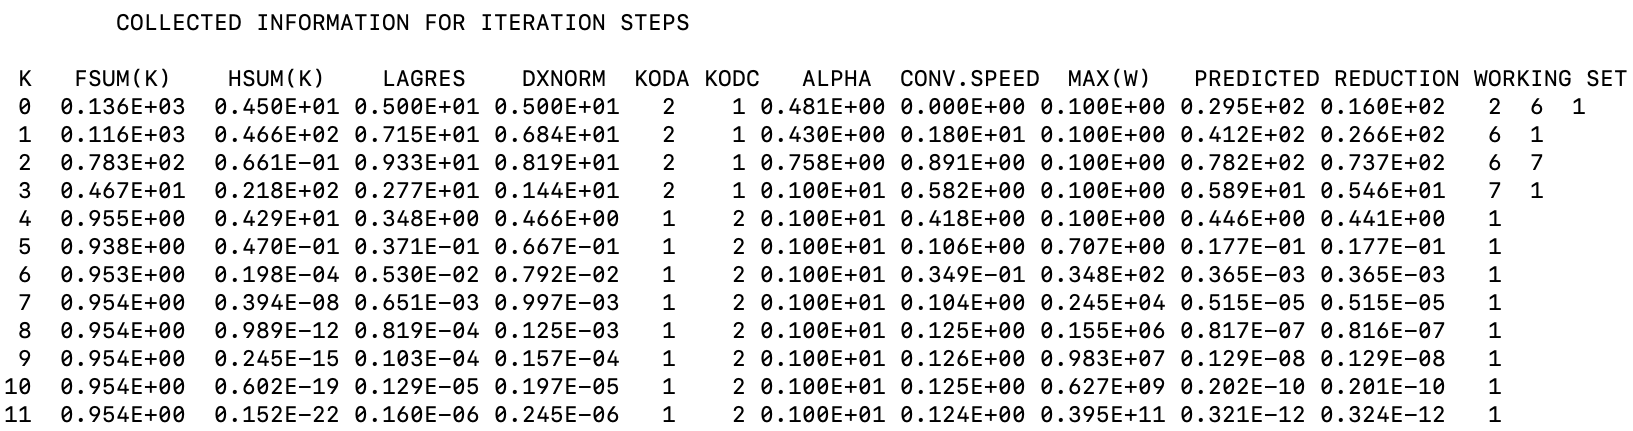
\includegraphics[scale=0.55]{FichiersSource/Images/sortie_f77_pb65}
    \caption{Itérations ENLSIP--Fortran sur le Pb65}
    \label{fig:iter fortran}
\end{figure}

\begin{figure}[ht]
    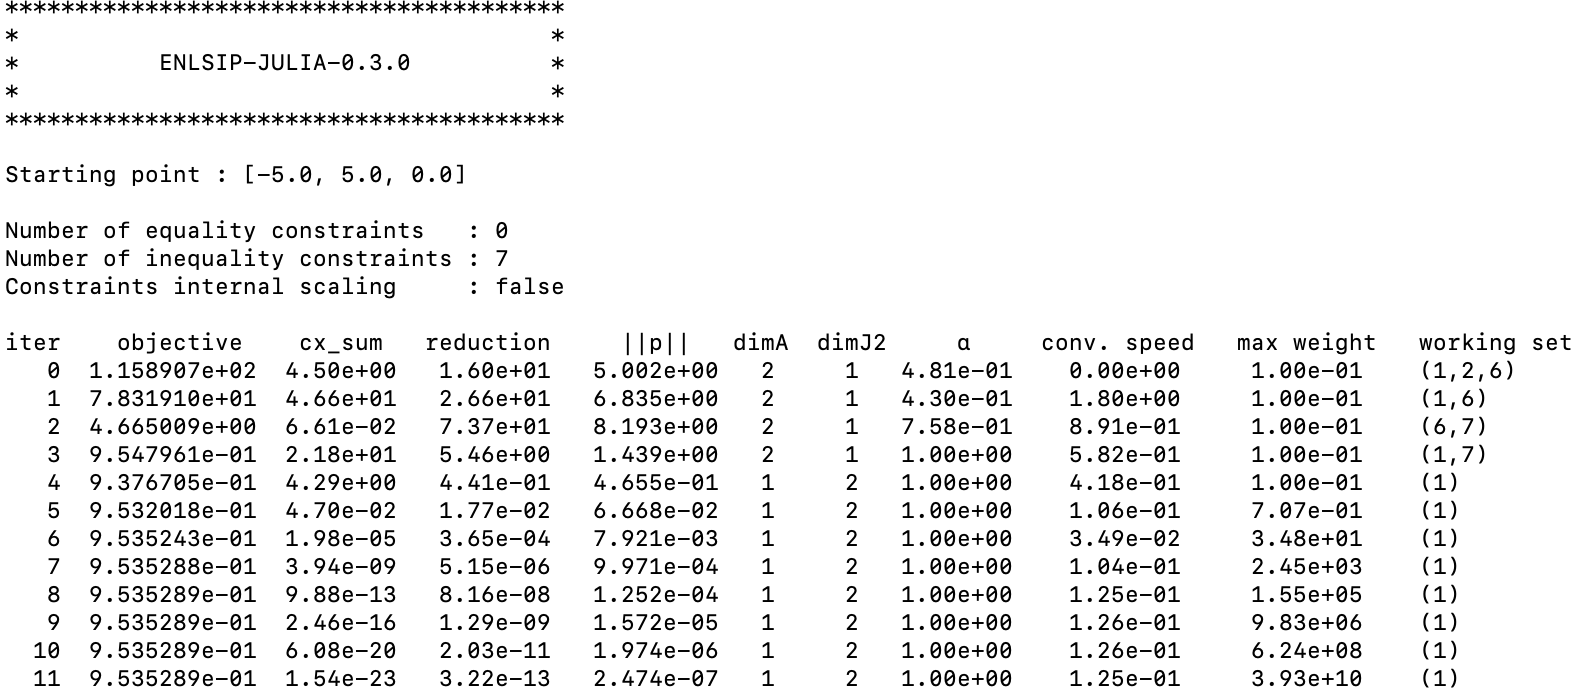
\includegraphics[scale=0.57]{FichiersSource/Images/sortie_pb65_julia}
    \caption{Itérations ENLSIP--Julia sur le Pb65}
    \label{fig:iter julia}
\end{figure}



On observe une concordance exacte des résultats intermédiaires obtenus et du nombre d'itérations effectuées. Cela prouve la bonne retranscription de 
la méthode, tout du moins sur ce problème. De futurs tests, réalisés à partir de modèles d'\HQ, permettront probablement de tirer de nouvelles conclusions à ce sujet.


\subsection{Comparaison des résultats et performances avec le solveur IPOPT}\label{compa_ipopt}

En plus du problème 65 déjà présenté, deux autres problèmes, le 57 et le 42 de la collection de~\citet{hockschi}, ont été utilisés afin de comparer les performances d'ENLSIP en Julia avec IPOPT.
Leurs modélisations et informations sont données respectivement en~\eqref{pb57} et en~\eqref{pb42}.

Commençons par la description du problème 57:

\begin{equation}\label{pb57}
 \left\{  
\begin{aligned} 
&\min f(x)= \sum\limits_{i=1}^{44} f_i(x)^2,\\ 
&\text{s.c.}\\
&0.49x_2-x_1x_2-0.09 \geq 0,\\
&x_1\geq 0.4,\  x_2 \geq -4.
\end{aligned} \right. 
\end{equation}

\begin{description}
    \item[Point initial] $x_0 = (0.42,5)^T$;
    \item[Solution attendue] $x^* = (0.419952675,1.284845629)^T$;
    \item[Fonction objectif à la solution] $f(x^*) =0.02845966972$,
\end{description}

avec $f_i(x) = b_i - x_1 - (0.49-x_1)\exp(-x_2(a_i-8)) \text{ pour }i=1,\ldots,44$. 

Les fonctions $f_i$ peuvent s'interpréter comme la différence entre l'observation $b_i$ et la prédiction du modèle de paramètres $x_1$ et $x_2$ réalisée en $a_i$.
Bien que cela reste un problème théorique, sa forme est bien adaptée au cas d'utilisation chez \HQ de l'algorithme ENLSIP. On peut s'attendre à une convergence vers la solution en un nombre plus faible 
d'itérations qu'avec IPOPT.

Les valeurs des données sont fournies dans l'ouvrage~\cite{hockschi}.

On remarque que le point initial est relativement proche de la solution attendue, en particulier la première composante. Ce problème s'est donc avéré être également un bon moyen de tester la robustesse de mon implémentation.

Passons désormais à la description du problème 42:

\begin{equation}
    \label{pb42}
\left\{  
\begin{aligned} 
&\min\ f(x)=(x_1-1)^2+(x_2-2)^2+(x_3-3)^2+(x_4-4)^2, \\ 
&\text{s.c.}\\
&x_1-2 = 0,\\
&x_3^2+x_4^2-2= 0.
\end{aligned} \right.
\end{equation}

\begin{description}
    \item[Point initial] $x_0 = (1,1,1,1)^T$;
    \item[Solution attendue] $x^* = (2,2,0.6\sqrt 2, 0.8\sqrt 2)^T$;
    \item[Fonction objectif à la solution] $f(x^*) =28-10\sqrt 2\approx 13.8578643$.
\end{description}

Le problème 42 peut sembler plus simple que les deux autres. Par exemple, la première contrainte impose directement la valeur du paramètre à l'optimum $x_1$.
Il présente néanmoins l'intérêt de n'avoir que des contraintes d'égalité et de partir d'un point non réalisable, ce qui permet d'éprouver la capacité de l'algorithme
à gérer ce genre de configurations.

Les différents tests ayant amené aux résultats présentés dans les tableaux~\ref{resultats:pb57},~\ref{resultats:pb42} et~\ref{resultats:pb65} ont été réalisés sur un ordinateur équipé d'un 
processeur IntelCore i5 de 10ème génération. La version $1.6.0$ de Julia a été utilisée et les temps de calcul ont été mesurés à l'aide de la librairie Julia \texttt{BenchmarkTools}. 

Le temps d'exécution n'a néanmoins pas pu être évalué sur ENLSIP-Fortran77.

\begin{table}
    \centering
    \begin{tabular}{|l|c|c|c|}
        \hline
        Solveur & Itérations & Temps de calcul &  Objectif \\ \hline
        ENLSIP-Julia & $5$ & $1.663\sec$ & $2.845966972\text{e-}02$ \\\hline
        IPOPT & $24$ & $2.003\sec$ & $2.845966907\text{e-}02$\\ \hline
    \end{tabular}  
    \caption{Comparaison d'ENLSIP-Julia avec IPOPT sur le problème 57}
    \label{resultats:pb57}
\end{table}

\begin{table}
    \centering
    \begin{tabular}{|l|c|c|c|}
        \hline
        Solveur & Itérations & Temps de calcul &  Objectif \\ \hline
        ENLSIP-Julia & $15$ & $1.493\sec$ & $1.385786438\text{e+}01$ \\\hline
        IPOPT & $10$ & $1.584\sec$ & $1.385786437\text{e+}01$\\ \hline
    \end{tabular}  
    \caption{Comparaison d'ENLSIP-Julia et IPOPT sur le problème 42}
    \label{resultats:pb42}
\end{table}

\begin{table}
    \centering
    \begin{tabular}{|l|c|c|c|}
        \hline
        Solveur & Itérations & Temps de calcul &  Objectif \\ \hline
        ENLSIP-Fortran77 & $11$ & -- & $0.953529\text{e+}01$ \\\hline
        ENLSIP-Julia & $11$ & $1.585\sec$ & $0.953528856\text{e+}01$\\\hline
        IPOPT & $12$ & $2.372\sec$ & $0.953528856\text{e+}01$\\ \hline
    \end{tabular}  
    \caption{Comparaison d'ENLSIP avec IPOPT sur le problème 65}
    \label{resultats:pb65}
\end{table}


Plusieurs constats peuvent être tirés de ces résultats. Tout d'abord, les minima trouvés par les deux algorithmes sont extrêmement proches, voire quasiment identiques, 
les différences apparaissant à partir de la huitième ou neuvième décimale selon les problèmes. L'objectif de parvenir à trouver des résultats corrects avec l'implémentation en Julia
d'ENLSIP semble donc globalement atteint.

En termes de performances, les temps de calcul d'ENLSIP-Julia remplissent largement les exigences fixées au chapitre~\ref{Besoins} et sont du même ordre de grandeur
que ceux d'IPOPT. Ce dernier point s'explique sûrement par le fait que les problèmes testés sont de très petite dimension et ne permettent donc pas de tirer des conclusions sur les différences 
de vitesse d'exécution. 

Ces premiers résultats se révèlent donc très encourageants pour la suite du développement d'ENLSIP en Julia.
Comme dit précédemment, d'autres tests seront réalisés sur des problèmes en plus grande dimension afin de se rapprocher petit à petit des problèmes effectivement résolus par l'outil 
de prévision dont \HQ\ se sert en production. % Commentaires sur l'implémentation en Julia 
\chapter*{Conclusion}\addcontentsline{toc}{chapter}{Conclusion}\label{Conclusion}
\markright{Conclusion}

\`A la fin de mon temps de stage, je suis parvenu à retranscrire l'algorithme ENLSIP en Julia. Ce travail s'est avéré prendre plus de temps que prévu, 
tant l'analyse du code source écrit en Fortran77 s'est avérée de plus en plus complexe à mesure que mon travail avançait. 

Les premiers tests effectués ont principalement contribué à mettre en avant la bonne retranscription en Julia 
de l'algorithme initialement codé en Fortran77. Cette implémentation bénéficie déjà des avantages de Julia en terme d'utilisation de librairies et de meilleure 
lisibilité du code. Néanmoins, les gains potentiels en terme de performances n'ont pas pu être évalués spécifiquement avec les tests réalisés sur des problèmes 
en relativement petite dimension.

La retranscription de l'algorithme n'étant pas complètement terminée, son accessibilité en tant que librairie Julia 
 n'a pas encore été entamée mais fait toujours partie des objectifs finaux du projet. 

Les prochains travaux seront dès lors consacrées à la mise en place de problèmes exploitant des données d'\HQ\ et faisant appel à des modèles
d'évaluation effectivement utilisés en production. Les tests réalisés apporteront de ce fait de nouveaux éléments de réponse quant à la pertinence du passage au langage Julia
pour les outils de prévision de la demande d'\HQ, et ce indépendamment des gains de lisibilité du Julia par rapport au Fortran77, ce qui est déjà un enjeu essentiel 
en terme de pérennité et de transmission des connaissances. 
Cette démarche permettra également de mettre l'implémentation réalisée dans des situations pouvant potentiellement mettre en difficulté la méthode d'optimisation utilisée par ENLSIP, 
contrairement aux cas relativement simples vus précédemment. 
 Cela pourrait potentiellement révéler de nouveaux bogues non détectés jusqu'à présent ou des portions de code mal retranscrites, notamment tout ce qui a trait à la gestion des erreurs.
 Leur correction pourrait évidemment perfectionner l'algorithme. 
 
 Un autre point à aborder concerne à la réalisation de tests sur un échantillon plus important de solveurs de programmation non linéaire. 
 Ainsi, l'on pourra comparer avec plus de pertinence l'efficacité d'ENLSIP face à des algorithmes plus modernes. 

Le projet sur lequel j'ai travaillé a aussi pour finalité de fiabiliser et moderniser des outils de prévision de la demande actuellement en production chez 
Hydro-Québec, ce qui constitue le second grand objectif du projet après celui consistant à retranscrire en Julia ENLSIP-Fortran77 et à valider le nouveau codage sur des problèmes jouets. 
Ces deux objectifs n'ont pas pu être 
traités en parallèle puisque la complétion du premier objectif était la condition nécessaire de réalisation du second. 
En outre, la retranscription en Julia a tout compte fait occupé la quasi-totalité de mon stage, tant l'analyse de 
l'algorithme codé en Fortran77 s'est révélée plus complexe et longue que prévu. De plus, perfectionner la méthode requiert déjà de mettre en exergue les points
devant être améliorés. Ceci ne peut être fait autrement qu'en confrontant ENLSIP à d'autres algorithmes d'optimisations déployant des méthodes plus actuelles.
Certains points d'amélioration ont néanmoins pu être discutés au travers de mes échanges avec mon maître de stage.

Un premier aspect pouvant être investigué concerne la gestion des contraintes. L'approche EQP développée dans ENLSIP amène à restreindre le nombre de contraintes 
traitées et à ne travailler qu'avec des égalités, ce qui se révèle avantageux dans le cadre des moindres carrés. Néanmoins, les avancées récentes dans les approches de type
primal-dual, tel que celle présentée par~\citet{andreas02} et adoptée dans IPOPT, permettent de mieux tirer parti de la totalité des contraintes et des multiplicateurs de Lagrange, améliorant grandement la convergence.
Cela est d'autant plus le cas lorsque l'on se situe proche de la solution, configuration où ENLSIP peut être amélioré et bénéficier de ce type de travaux. On remarque par exemple sur la 
figure~\ref{fig:iter julia} que les cinq dernières itérations ne modifient la fonction objectif qu'à partir de la huitième décimale, ce qui a en réalité peu d'impact sur la solution obtenue.

Un autre aspect traite du calcul de la longueur de pas. La méthode décrite par~\citet{lindstromwedin1984}, développée dans les années 1980, présente des 
caractéristiques pouvant s'apparenter aux méthodes de régions de confiance~\cite{conngoultoin00}. L'idée d'approcher la fonction objectif pénalisée afin de calculer 
des valeurs de pas de plus en plus affinées est en effet commune aux deux approches. Agrémenter le calcul du pas d'une méthode de ce type pourrait donc également s'avérer pertinent en vue de la 
modernisation d'ENLSIP.

En somme, la modernisation de la méthode d'optimisation d'ENLSIP proprement dite pourra faire l'objet de futurs projets de recherche pour \HQ\ et l'UdeM.
 % Conclusion 

%%%%%%%%%%%%%%%%%%%%%%%%%%%%%%%%%%%%%%%%%%%%%%%%%%%%%%


%%%%%%%%%%%%%%%%%%%%%%%%%%%%%%%%%%%%%%%%%%%%%%%%%%%%%%
% Accronymes
%%%%%%%%%%%%%%%%%%%%%%%%%%%%%%%%%%%%%%%%%%%%%%%%%%%%%%




%%%%%%%%%%%%%%%%%%%%%%%%%%%%%%%%%%%%%%%%%%%%%%%%%%%%%%
% Bibliographie
%%%%%%%%%%%%%%%%%%%%%%%%%%%%%%%%%%%%%%%%%%%%%%%%%%%%%%

%\thispagestyle{fancy}
\bibliographystyle{plainnat-fr} 
\bibliography{biblio}
% Le style est mis entre accolades.
\thispagestyle{fancy}
\addcontentsline{toc}{chapter}{\textmd{Bibliographie}}

%%%%%%%%%%%%%%%%%%%%%%%%%%%%%%%%%%%%%%%%%%%%%%%%%%%%%%
% Annexes
%%%%%%%%%%%%%%%%%%%%%%%%%%%%%%%%%%%%%%%%%%%%%%%%%%%%%%

\appendix
\chapter*{Annexes}\label{Annexes}
\markright{Annexes}
\addcontentsline{toc}{chapter}{Annexes}

\section*{Définition des composantes du calcul des pénalités}

On rappelle:
\begin{itemize}
    \item $z=\left[(\nabla \hc_i(x_{k})^Tp_{k})^2 \right]_{1 \leq i \leq t}$ 
    \item $\mu =  \left[\dfrac{|(J_{k}p_{k})^Tr(x_k) + \|J_{k}p_{k}\|^2|}{\delta} - \|J_{k}p_{k}\|^2 \right]$ $(\delta=0.25)$
    \item $t$ est le nombre de contraintes actives à l'itération $k$
    \item $\omega_1$ est la dimension utilisée dans le calcul du premier membre de $p_k$ la direction de descente(voir~\ref{direction_descente})
\end{itemize}

\begin{enumerate}
    \item
    Si $z^{T}\hat{w}^{(old)} \geq \mu$
     
     \begin{algorithmic}
     \STATE{$\tau = 0$}
     \FOR{$i=1:t$}
     \STATE{$e=\nabla \hc_i(x_{k})^Tp_{k}(\nabla \hc_i(x_{k})^Tp_{k}+\hc_{i}(x_{k}))$}
     \IF{$e > 0$}
     \STATE{$y_{i}=e$}
     \ELSE
    \STATE{$\tau = \tau - e*\hat{w}_{i}^{(old)}$, $y_{i}=0$}
     \ENDIF
     \ENDFOR
     \end{algorithmic}
     
     \item
    Si $z^{T}\hat{w}^{(old)} < \mu$ et $\omega{1}\neq t$
    
     \begin{algorithmic}
     \STATE{$\tau = \mu$}
     \FOR{$i=1:t$}
     \STATE{$e=-\nabla \hc_i(x_{k})^Tp_{k}*\hc_{i}(x_{k})$}
     \IF{$e > 0$}
     \STATE{$y_{i}=e$}
     \ELSE
    \STATE{$\tau = \tau - e*\hat{w}_{i}^{(old)}$, $y_{i}=0$}
     \ENDIF
     \ENDFOR
     \end{algorithmic}
     
   Dans les deux cas ci-dessous, la première contrainte du problème~\ref{pb poids} est $y^{T}\hat{w} \geq \tau$.
    
    \item
    Si $z^{T}\hat{w}^{(old)} < \mu$ et $\omega_{1}= t$
    \begin{algorithmic}
        \STATE $y = z$ et $\tau = \mu$ 
    \end{algorithmic}
    
    Et la première contrainte du problème~\ref{pb poids} est $y^{T}\hat{w} = \tau$.
    
    \end{enumerate}
     
\begin{algorithm}
  \centering
  \begin{algorithmic}
    \STATE{\textbf{function} goldstein\_armijo\_step}
    \STATE{$\alpha=\alpha_{0}$}
    \WHILE{$\phi(\alpha) \geq \phi(0) + \gamma * \alpha* \phi^{\prime}(0)$ \AND ($\alpha \|p_{k}\| > \varepsilon_{rel}$ \OR $\alpha > \alpha_{min}$)}
    \STATE{$\alpha = \alpha /2$}
    \ENDWHILE
    \RETURN{$\alpha$}
    \COMMENT{\textit{Les constantes $\varepsilon_{rel}$ et $\gamma$ désignent respectivement la racine carrée de la précision machine sur les nombres 
        flottants et une constante valant $0.25$ en pratique}}
  \end{algorithmic}
  \caption{Calcul de longueur de pas avec une méthode de type Armijo-Goldstein} 
    \label{fig:armijo}
\end{algorithm}








  
\end{document}

%%%%%%%%%%%%%%%%%%%%%%%%%%%%%%%%%%%%%%%%%%%%%%%%%%%%%%
% FIN DOCUMENT
%%%%%%%%%%%%%%%%%%%%%%%%%%%%%%%%%%%%%%%%%%%%%%%%%%%%%%
